\documentclass[11pt,a4paper]{article}

\usepackage{amsmath}
\usepackage[a4paper,includehead]{geometry}

\usepackage{graphicx} % Required for inserting images
\usepackage{tabularx}
\usepackage{natbib}
\usepackage[spaces,hyphens]{url}
\usepackage[hidelinks]{hyperref}
\usepackage{setspace}
\usepackage{booktabs}
\usepackage{hyphenat}
\usepackage{color}
%\usepackage{subfig}
% \usepackage[justification=left,hang]{caption}
\usepackage[justification=raggedrig,hang]{caption}
\usepackage{subcaption}
	%\captionsetup[subfigure]{labelfont=normal,textfont=normalfont,singlelinecheck=off,justification=centering}
\usepackage[table]{xcolor} 
\usepackage{colortbl}
\usepackage[hang]{footmisc}
\usepackage{appendix}
\usepackage{float}

\geometry{left=2.25cm,right=2.25cm,top=1.5cm,bottom=2cm}
%\hyphenation{EMU} \hyphenation{CEECs}
%\setlength{\parindent}{0pt} \setlength{\parskip}{10pt} %\setlength{\abovecaptionskip}{-5pt}
%\setlength{\belowcaptionskip}{-5pt} \setlength{\floatsep}{10pt}
\clubpenalty = 10000 
\widowpenalty = 10000
\displaywidowpenalty = 10000

% \makeatletter
% \setlength{\@fptop}{5pt} %setzt den abstand der floats vom oberen Rand auf Null- 5 entspricht der gleichen Höhe wie die wo der Text anfängt
% 		%\setlength\@fptop{0\p@ \@plus 1fil}
% \setlength\@fpsep{10pt plus 2pt minus 2pt} %Abstand zwischen den Floats
% \makeatother



%%%%%%%%%%%%%%%%%%%%%%%%%%%%%%%
\begin{document}
\setlength{\abovedisplayskip}{2cm}
\setlength{\abovedisplayshortskip}{2cm}
\setlength{\belowdisplayskip}{0cm}
\setlength{\belowdisplayshortskip}{2cm} %Abstand zwischen Text und Formel




\title{Smooth and Persistent Forecasts of German GDP}
\author{Katja Heinisch\thanks{Halle Institute for Economic Research (IWH).} \hspace{0.2cm}
Simon van Norden\thanks{HEC Montréal and CIREQ.} \hspace{0.2cm}
Marc Wildi\thanks{Zurich University of Applied Sciences (ZHAW).}}
\date{May 2025 \\
\vspace{2cm} \textit{Work in progress, not for circulation}}



\maketitle
%%%%%%%%%%%%%%%%%%%%%%%
\maketitle

\begin{abstract} %max.
This paper addresses the trade-off between informational efficiency and forecast smoothness in economic forecasting. Efficient forecasts are often volatile, limiting their practical usefulness. We propose a novel method that employs the framework of Multivariate Smooth Sign Accuracy (M-SSA) to extract smoothed components from leading indicators. This approach enhances the signal-to-noise ratio and allows for systematic control over forecast volatility and timing. Applied to German GDP, our method yields smoothed forecasts that improve the accuracy of traditional models, particularly over medium-term horizons. While smoother forecasts may lag slightly, this can be mitigated by adjusting the forecast horizon. Our findings offer practical tools for forecasters and policymakers subject to adjustment costs or frictions in updating forecasts or implementing policy changes.

\end{abstract}

\bigskip \vspace{10pt}
\textbf{Keywords:} Forecast Smoothing, Smooth Sign Accuracy 
\newline
\textbf{JEL Classification:} C53, E37, E66
%C53 – Forecasting and Prediction Methods; Simulation Methods
%E37 – Forecasting and Simulation: Models and Applications
%E66 – General Outlook and Conditions: Forecasts and Simulations
\thispagestyle{empty}


\onehalfspacing
%\doublespacing
\renewcommand{\thepage}{\arabic{page}} \setcounter{page}{1}
\newpage
\section{Motivation}\label{sec:motivation}

\begin{quote}
     \quad ``As we parse the incoming information, we are focused on separating the signal from the noise as the outlook evolves.''\\
    \textit{Speech by Federal Reserve Board Chair Jerome H. Powell, March 07, 2025, \\
    University of Chicago Booth School of Business}
\end{quote}

Economic forecasters face a dilemma: While efficiency suggests that their forecasts should incorporate all available information, the resulting forecasts are often volatile, which may reflect greater information content or contamination by excessive ``noise''. Further, forecast users (including public and private decision makers) may be constrained by how rapidly they can adjust to changing forecasts.\footnote{For example, private or public spending decisions may be constrained by annual budgets. Similarly, central banks increasingly attempt to smooth interest rate changes to allow them to signal the future direction of policy to markets, while private firms attempt to smooth changes in dividends.}

%%% Further recent literature
% \cite{lehmann2021predicting} show the performance of ifo busines cycles indicator for the nowcast (h=0) and forecast (h=1) 

\cite{Wildi2024,Wildi2025} and \cite{McElroy2019,McElroy2020} propose novel methods that optimally smooth forecasts by controlling the expected frequency of sign changes. The resulting Smooth Sign Accuracy (SSA) framework encompasses efficient mean-square error (MSE) as a special case and produces increasingly smooth forecasts as changes in forecast sign are increasingly penalized. 

% First, direct AR-forecast (benchmarks) are fairly noisy. In contrast,
% trend forecast are generally (substantially) smoother
% Second, zero-crossings are possibly indicative of relevant changes in
% the economy (trend growth cycle) and the rate of
% zero-crossings can be controlled by SSA.
% Third, trend forecasts and direct AR forecasts are similar with
% respect to mean-square error (forecast) performances
% Fourth, lead/lag and smoothness can be controlled (simultaneously
% up to some point) by SSA:
% Finally, multivariate designs can provide added value.



This study proposes a methodological innovation that extends the classical direct forecasting framework by integrating dimension-reduced information extracted through Multivariate Smooth Sign Accuracy (M-SSA). The core idea is to replace raw
%, unprocessed 
leading indicators with smoothed and filtered components derived from the M-SSA procedure, thereby improving the signal-to-noise ratio in the predictor variables used to forecast GDP. We apply this framework to well-established German economic indicators to show its ability to improve forecasts of GDP and GDP trends using a variety of sample periods and performance metrics. 

Surprisingly, we find that smoothing indicator-based forecasts often provides useful leading information for GDP, especially over mid-term horizons ranging from two to four quarters ahead. We also show that while smoother GDP forecasts lag efficient MSE forecasts slightly, this can be mitigated by adjustments in the forecast horizon.\footnote{The lag reflects the trilemma highlighted by \cite{McElroy2019} in which forecasters choose between forecast accuracy, timeliness and volatility.}



%Previous research often highlights the utility of direct forecasts, particularly for short-term predictions such as nowcasting and forecasts one quarter ahead. However, this paper advances the literature by showing that more sophisticated predictors—specifically, filtered components obtained via M-SSA yield superior performance, especially over mid-term horizons ranging from two to four quarters ahead.

Section \ref{sec:data} describes our data series, the sample period used, and documents their dynamic behaviour. Section \ref{sec:direct_forecast} provides benchmark forecasts using simple direct projections of GDP based on our indicators. We demonstrate how in-sample forecast performance may improve when we ``de-noise'' the indicators prior to projection with simple smoothing filters. Section \ref{sec:mSSA} defines the M-SSA method and shows how its forecast performance compares to that of direct projections as well as how it varies with forecast horizon. Section \ref{sec:mSSA_component} considers the ability of our indicators to forecast German GDP growth using the M-SSA framework, and Section \ref{sec:revisions} investigates the temporal stability of the estimated forecasting equations. Section \ref{sec:conclusions} summarizes the results and concludes. The Appendix provides some additional results. 



\section{Data and Dependence}\label{sec:data}
\subsection{Data}
The analysis employs a set of well-established leading indicators to forecast quarterly German GDP \citep{Drechsel2012financial,Heinisch2018bottom}, including industrial production (IP), the ifo Business Climate Index (ifo\_c), the Economic Sentiment Indicator (ESI), and the term spread between 10-year bond yields and the 3-month EURIBOR rate (spre\_10y\_3m) covering the period 1995 to 2024.  
We take into account the publication lag of the indicators and the GDP series.\footnote{Data revisions are not considered, given that previous studies \citep{Heinisch2019} have shown that their overall effect on forecast performance is minor.} 
While GDP is available with a one-quarter delay (published in mid of the next quarter), and IP is released with a one-month lag, business surveys and financial data are published without any lag, see Table \ref{tab:data_stucture} which presents the data structure as of the end of January 2025, just before the publication of the Flash estimate for the previous quarter.\footnote{Starting in the second quarter of 2020, the German Federal Statistical Office published for the first time the gross domestic product (GDP) 30 days after the end of the quarter.} All series are consequently re-aligned to correspond with the information available to forecasters, with GDP and IP variables shifted forward according to their respective lags. Table \ref{tab:data_stucture_aligned} displays the dataset as of the end of 2024, with GDP and IP variables temporally aligned at the sample endpoint. This configuration reflects the matrix of explanatory variables accessible in Q4-2024 for the purposes of nowcasting or forecasting GDP. For illustrative purposes, an additional target column is included on the right side of the table, representing the dependent variable for nowcasting applications. In the case of an $h$-step ahead forecast, this column is shifted upwards by $h$ quarters. 


\begin{table}[ht]
\centering
\begin{tabular}{rrrrrr}
  \hline
 & GDP & ip & ifo\_c & ESI & spr\_10y\_3m \\ 
  \hline
2024-07-01 &  & 90.700 & 85.800 & 92.500 & -1.300 \\ 
  2024-08-01 &  & 93.200 & 84.900 & 90.900 & -1.400 \\ 
  2024-09-01 &902.571  & 91.200 & 83.700 & 89.800 & -1.400 \\ 
  2024-10-01 &  & 90.800 & 84.100 & 90.700 & -1.200 \\ 
  2024-11-01 &  & 92.200 & 83.800 & 89.300 & -0.900 \\ 
  2024-12-01 &  &  & 82.800 & 86.900 & -0.800 \\ 
  2025-01-01 &  &  & 82.500 & 88.100 & -0.200 \\ 
   \hline
\end{tabular}
\caption{Ragged end as of January 2025, before publication of the flash estimate.} 
\label{tab:data_stucture}
\end{table}










\begin{table}[ht]
\centering
\begin{tabular}{rrrrrrrc}
  \hline
 & GDP & ip & ifo\_c & ESI & spr\_10y\_3m &&Target (nowcast)\\ 
  \hline
  2024-07-01 & & 93.400 & 85.800 & 92.500 & -1.300&|& \\ 
  2024-08-01 & & 90.700&  84.900 & 90.900 & -1.400&| &\\ 
  2024-09-01 & 901.623 &93.200 & 83.700 & 89.800 & -1.400&| &902.571\\ 
  2024-10-01 &  &91.200 & 84.100 & 90.700 & -1.200&| &\\ 
  2024-11-01 &  & 90.800& 83.800 & 89.300 & -0.900&| &\\ 
  2024-12-01 &902.571   & 92.200  & 82.800 & 86.900 & -0.800&| &?\\ 
    \hline
\end{tabular}
\caption{Columns 1 through 5 constitute the matrix of explanatory variables available in Q4-2024 for the establishment of a GDP nowcast or forecast. All series are artificially aligned at the sample endpoint. Column 6 represents the target variable for the nowcast in Q4-2024.} 
\label{tab:data_stucture_aligned}
\end{table}



To ensure comparability and mitigate scale effects, all indicators (except the spread, which is differenced only) are log-differenced and standardized, the latter applied solely for ease of visual inspection. Additionally, extreme outliers associated with the COVID-19 pandemic are trimmed to prevent distortions in subsequent figures. 
 Monthly series are transformed to quarterly series and are displayed in Figure \ref{fig:data}, while Figure \ref{fig:data_lags} offers a close-up view of the financial crisis and the pandemic.\footnote{Monthly series are averaged to quarterly values.} The latter figure illustrates that the real-time GDP and industrial production series are synchronized at dips and peaks (coincident), whereas the other indicators tend to lead somewhat. The latter can be leveraged in a multivariate approach to enhance forecasting performance compared to univariate benchmarks. 


\begin{figure}
  \begin{subfigure}[t]{0.49\textwidth}
    \centering
    \includegraphics[width=\linewidth]{./Figures/Data.pdf}
    \subcaption{Full Sample.}
    \label{fig:data}
\end{subfigure}
\hfill
\begin{subfigure}[t]{0.49\textwidth}
    \centering
    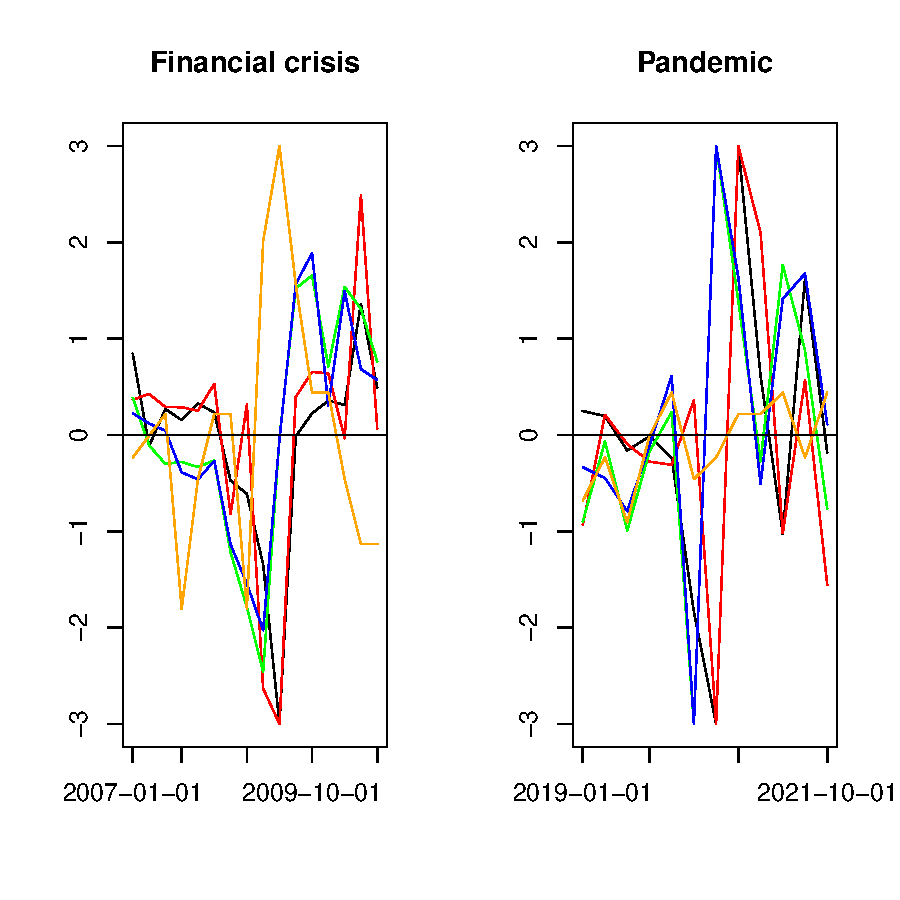
\includegraphics[width=\linewidth]{./Figures/data_lags.pdf}
    \subcaption{Leads \& lags during financial crisis \& Pandemic.}
    \label{fig:data_lags}
\end{subfigure}
\caption{GDP \& Indicators: standardized log-differences, trimmed to $\pm 3$ standard deviations.}
\end{figure}






%%%%%%%%%%%%%%%%%%% here comes the GIT-file

\subsection{Dependence}
To examine the dynamic interdependencies among the variables, we estimate their cross-correlations as well as their vector moving-average (VMA) representations. The latter is a key input to the multivariate filters we develop in Sections \ref{sec:mSSA} and \ref{sec:mSSA_component}. 

Figures \ref{CCF} (full sample) and \ref{CCF_wc} (omitting the Pandemic period) show the sample cross-correlation functions (CCF's) between current and lagged GDP and the two survey indicators. Both figures show strong correlations that peak at leads relative to GDP. Results for IP showed no lead, while correlations for the term spread were weaker. The figures also show that the precise strengths of the correlations are influenced by the outliers associated with the COVID-19 pandemic. In the interest of model stability, we exclude data from Q4-2019 to Q4-2020 (pandemic) when modelling the dynamics for the multivariate filters developed below. 

\begin{figure}[ht]
    \begin{subfigure}[htpb]{\textwidth}
        \begin{center}
            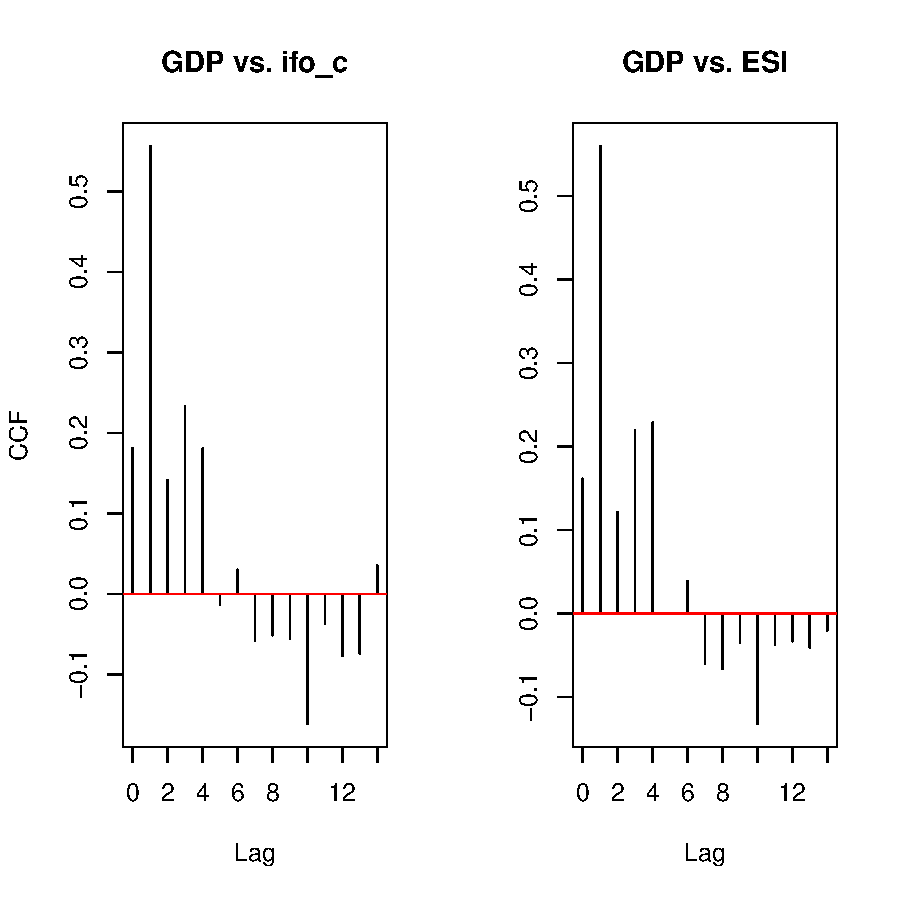
\includegraphics[height=3in, width=4.5in]{./Figures/CCF.pdf}
            \caption{Full data set from Q2-1991 to Q4-2024.\label{CCF}}
        \end{center}
    \end{subfigure}
    \\
    \begin{subfigure}[htpb]{\textwidth}
        \begin{center}
            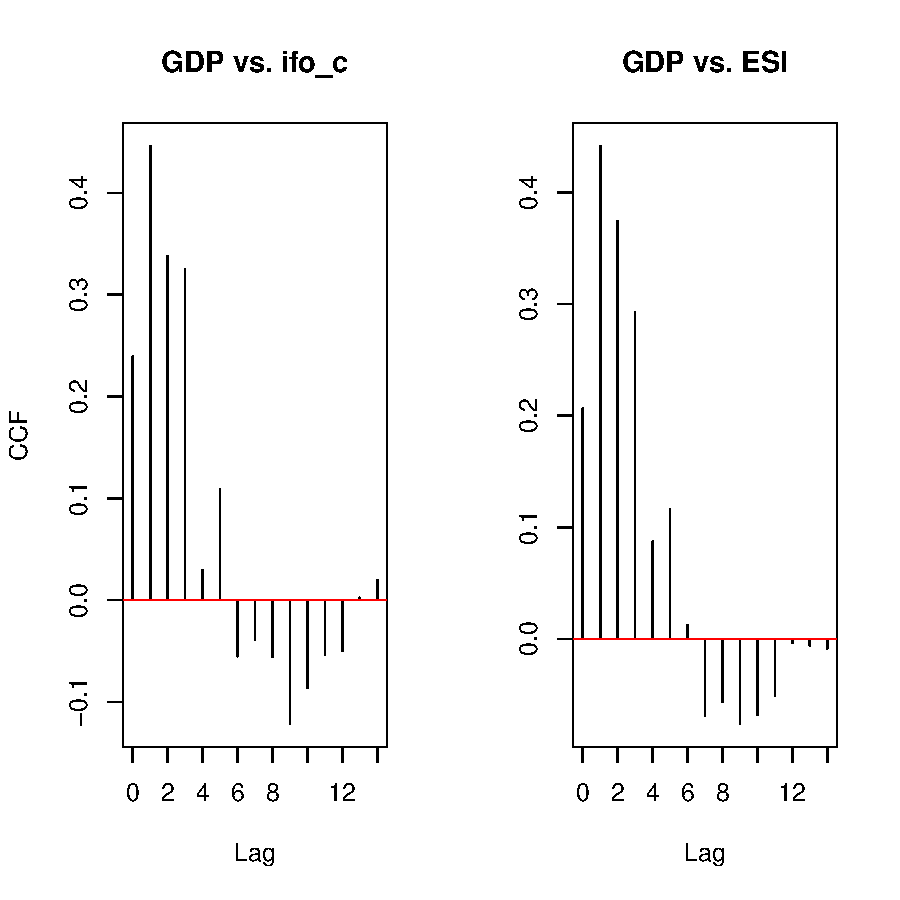
\includegraphics[height=3in, width=4.5in]{./Figures/CCF_wc.pdf}
            \caption{Without Pandemic (omitting Q4-2019 to Q4-2020).\label{CCF_wc}}
        \end{center}
    \end{subfigure}
    \caption{Sample cross-correlation functions (CCF) showing correlations with lags of GDP growth.}
\end{figure}

We then estimated a variety of parsimonious VARMA models to capture these dynamics, selecting parsimonious VAR(1) and VAR(3) specifications.\footnote{We used the \texttt{refVARMA()} procedure in the \cite{MTSpackage} \texttt{MTS} package, which sets VARMA coefficients with t-statistics below a critical threshold to zero \citep[see][]{tsay2013multivariate}.  This led to a VAR(1) specification with a threshold of 1.5. The VAR(1) left some residual evidence of higher-order dynamics, but capturing these in our limited sample size was difficult without overfitting. We therefore explored VAR($p$) models with coefficients estimated by Elastic Net using the \cite{ElasticNet} \texttt{elasticnet} package.  This led to a VAR(3) specification with 7 steps. For additional details, see \cite{ElasticNet} and the references therein.} The figures \ref{ma_inv_BIP} and \ref{ma_inv_BIP_var3_en} show the implied responses of GDP to shocks to each indicator variable.\footnote{Shown are the MA coefficients for GDP from the vector moving-average (VMA) models obtained by inversion of the VAR(1) and VAR(3) representations respectively (i.e. the impulse-response functions, or IRFs, of GDP to the correlated reduced-form shocks.)} 

%
%   SvN: I've added the following very brief description of Elastic-Net
%
% Linear regression models often suffer from issues such as overfitting and multicollinearity when the number of predictors exceeds the number of observations. Regularization techniques, such as ridge regression and the lasso, offer solutions by imposing penalties on model parameters. However, ridge regression maintains all predictors, while the lasso leads to sparse solutions by shrinking coefficients to zero. The elastic net estimator, introduced by \cite{ZouHastie2004JRSSB}, addresses limitations inherent in these approaches by blending their penalty functions.

% The elastic net estimator is obtained by solving the following optimization problem:

% \begin{equation}
% \hat{\beta}^{EN} = \arg\min_{\beta} \left( \sum_{i=1}^{n} (y_i - X_i \beta)^2 + \lambda_1 \sum_{j=1}^{p} |\beta_j| + \lambda_2 \sum_{j=1}^{p} \beta_j^2 \right),
% \end{equation}

% where $\lambda_1$ and $\lambda_2$ are non-negative tuning parameters, and $X_i$ represents the predictor variables.
% This formulation encompasses the least-squares estimator as the special case where $\lambda_1 = 0$ and the LASSO as the special case where $\lambda_2 = 0$. Unlike the lasso, which may arbitrarily select correlated predictors, the elastic net encourages grouping of strongly correlated variables. The combined penalties stabilize estimation in cases with high-dimensional predictors.
%
%
%

\begin{figure}[H]
    \begin{center}
        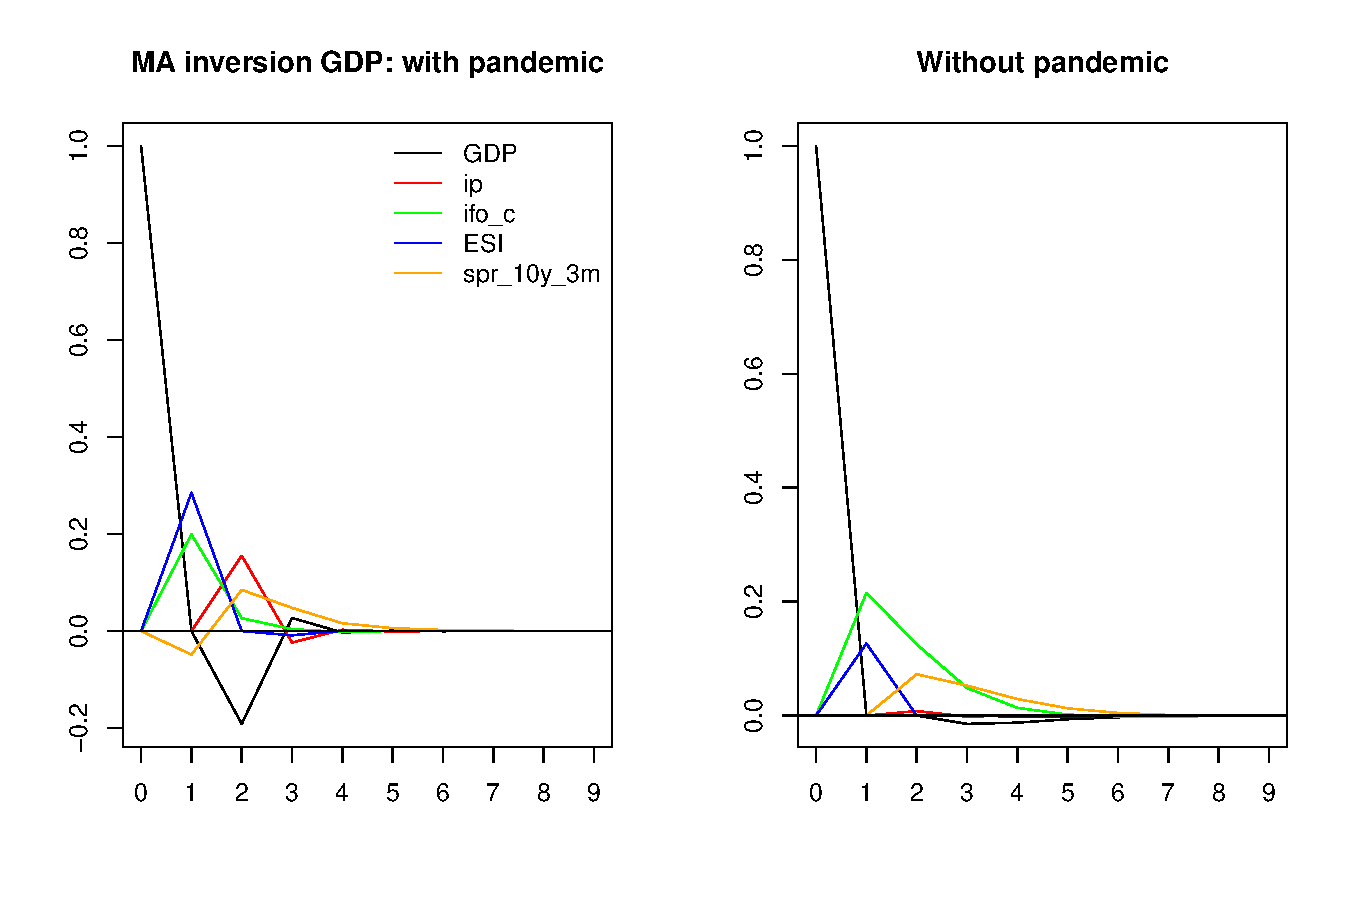
\includegraphics[height=3in, width=6in]{./Figures/ma_inv_BIP.pdf}
        \caption{VMA coefficients for GDP implied by VAR(1)\\Estimation with pandemic (left) and without pandemic (right).
        \label{ma_inv_BIP}}\end{center}
\end{figure}

\begin{figure}[H]
    \begin{center}
        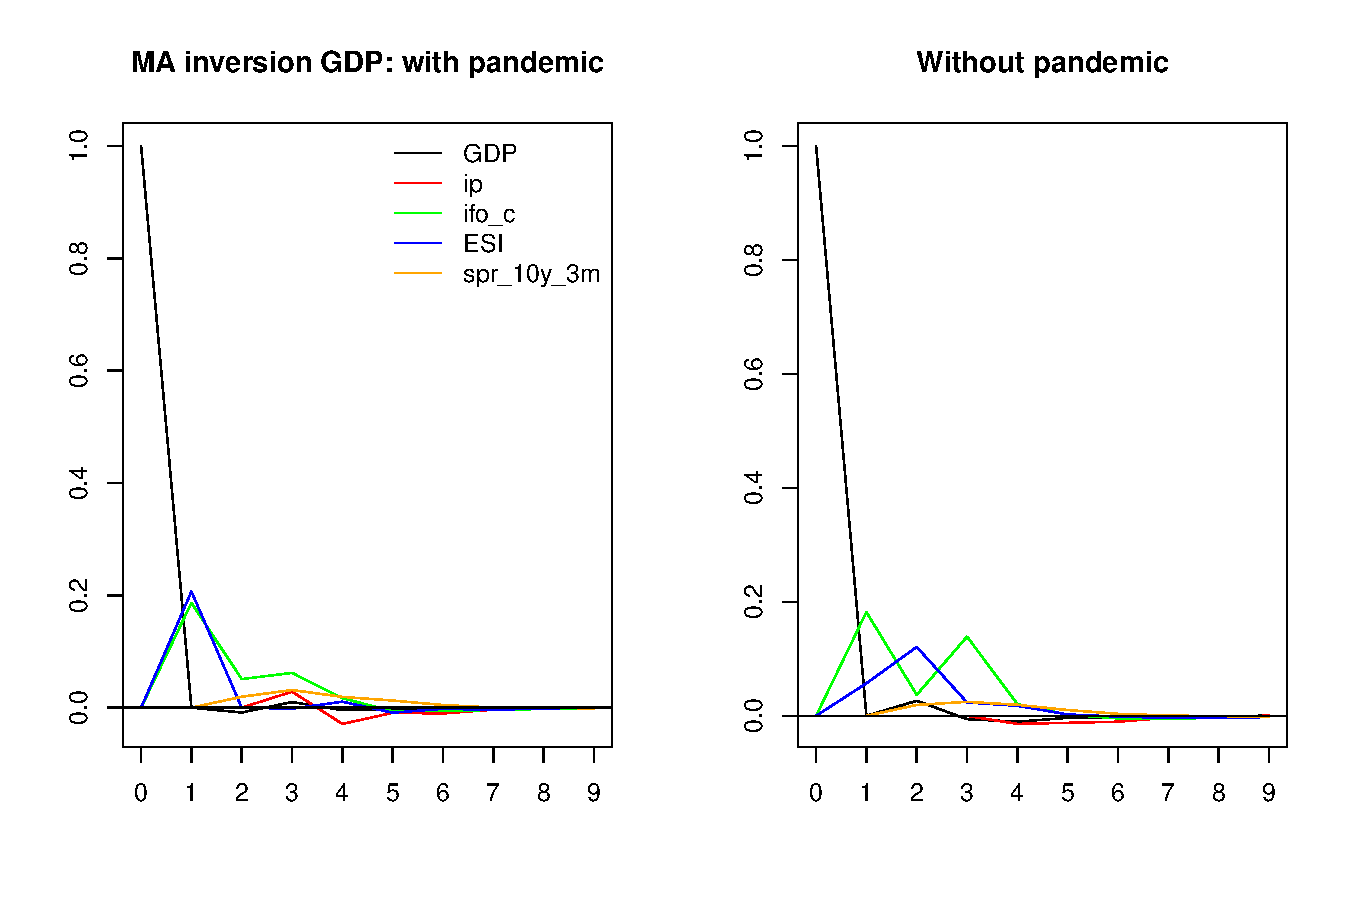
\includegraphics[height=3in, width=6in]{./Figures/ma_inv_BIP_var3_en.pdf}
        \caption{VMA coefficients for GDP implied by VAR(3)\\Estimation with pandemic (left) and without pandemic (right).
        \label{ma_inv_BIP_var3_en}}\end{center}
\end{figure}



%The models encapsulate key characteristics of the data after adjusting for publication lags. Notably, 
GDP exhibits the strongest response to shocks in the two survey indicators—ifo and ESI\footnote{There is also weaker evidence of a response to the term spread at longer lags.}. The impact of the pandemic modifies the lag structure by emphasizing shorter dependencies triggered by the alternating outliers during that specific episode. Removing the COVID-19 breakout from the analysis results in smoother, somewhat longer-tailed dependencies, consistent with the observed empirical autocorrelation functions. In particular, the VAR(3) model captures slightly extended lead times and more nuanced lag patterns\footnote{The VAR(3) model yields marginal improvements in multivariate filtering performance. However, due to its relative simplicity, this study primarily employs the VAR(1) model. The M-SSA package (accessible at \url{https://github.com/wiaidp/R-package-SSA-Predictor}) offers more advanced capabilities, including the implementation of the VAR(3) model and various additional (Bayesian) VAR specifications.}. The delayed response of GDP to movements in these indicators suggests that multivariate models could yield superior forecasting performance compared to univariate approaches, a hypothesis we explore in the next section


\section{Forecasts with Pre-Filtering}\label{sec:direct_forecast}

In this section, we demonstrate how pre-filtering indicator variables may improve the performance of simple forecasts by removing noise. For simplicity, all the models in this section are direct projections of GDP on our indicators and take the form

\begin{equation}
    u_{t+h} = \boldsymbol{\beta'} \cdot \mathbf{X}_t + \varepsilon_t
    \label{eq:direct_forecast}
\end{equation}

where
\begin{itemize}
    \item $u_{t+h}$ is the growth rate of GDP, $h = \{0, 1, 2, ... \}$
    \item $\mathbf{X}_t \equiv [1,u_{t-1}, ip_t, ifo\_c_t, ESI_t, spr\_10y\_3m_t]'$ or their transformed counterparts and $u_{t-1}$ accounts for the publication lag of GDP.\footnote{Including lagged GDP enables the nesting of the AR forecast within the broader modeling framework.}
    \item $\hat{\boldsymbol{\beta}}$ is estimated by least-squares, omitting observations affected by the pandemic, i.e. Q4-2019 to Q4-2020.
\end{itemize}

We then demonstrate how in-sample forecast performance improves when we ``de-noise'' the indicators prior to projection with simple smoothing filters.\footnote{The smoothing filters are one-sided (concurrent) filters of length 31, therefore, estimation of both forecasting models omits the first 30 observations.}

\subsection{Unfiltered Indicators}\label{cdf}

%So-called direct forecasts are obtained by regressing the relevant indicators on forward-shifted GDP, accounting for the additional publication lag. To illustrate the concept, we rely on all indicators and full sample information, excluding observations affected by the pandemic. In-sample forecasts and the forward-shifted GDP, which serves as the target, are presented in Figures \ref{direct_wc} (full dataset without the pandemic) and \ref{direct_wc_financial_crisis} (financial crisis) for forecast horizons up to three quarters ahead. 

\begin{figure}[H]
    \begin{center}
        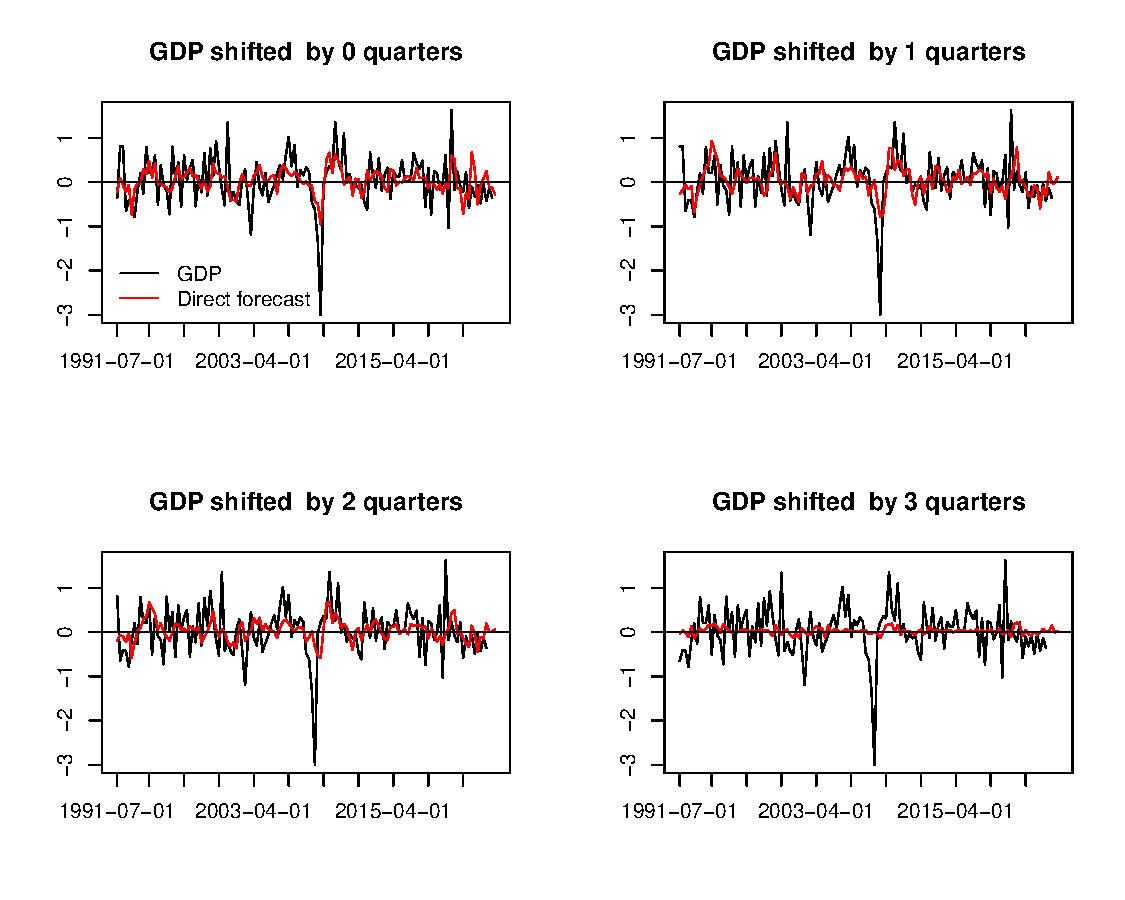
\includegraphics[width=0.9\textwidth]{./Figures/direct_wc_all.pdf}
        %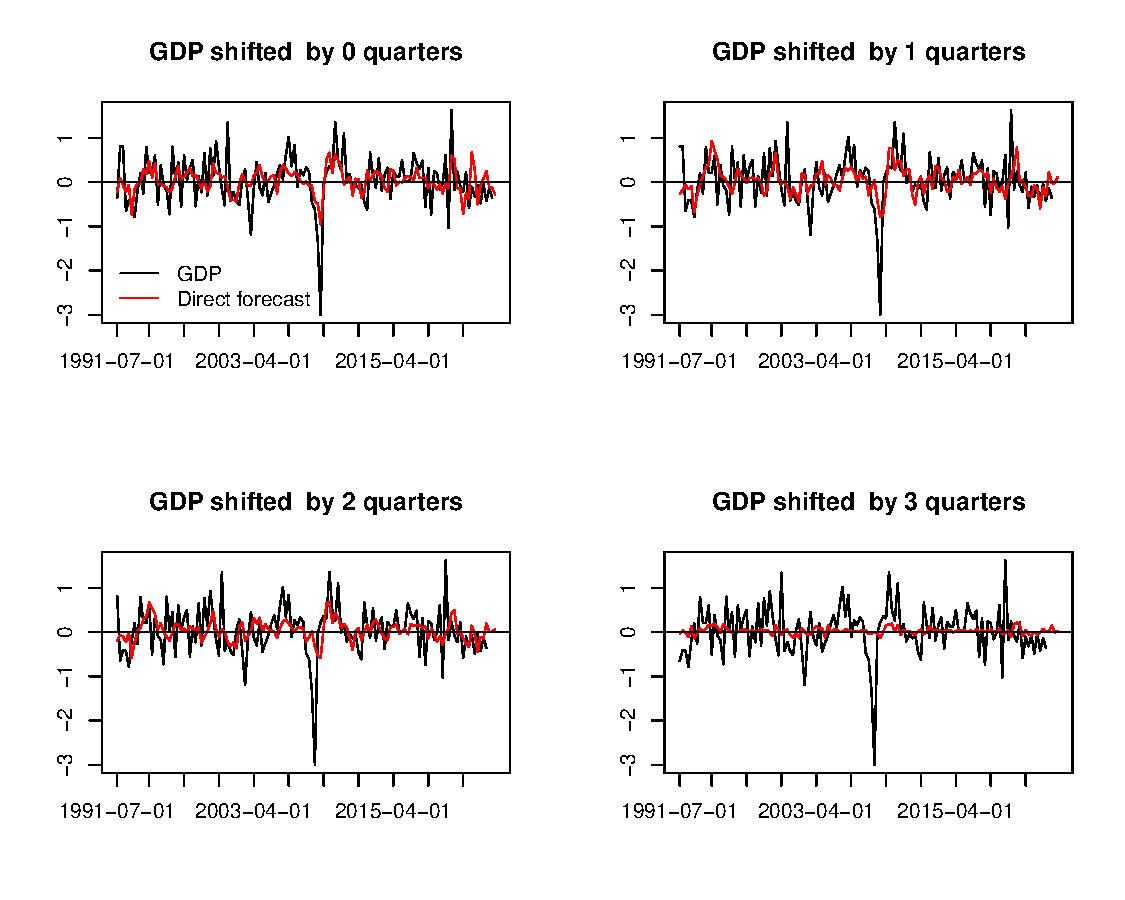
\includegraphics[height=3in, width=4.5in]{./Figures/direct_wc_all.pdf}
        \caption{Direct forecasts (red lines) based on all indicators and full sample information (without pandemic): GDP (black line) left-shifted  by zero, one, two, and three quarters.
        \label{direct_wc}}
    \end{center}
\end{figure}

Figures \ref{direct_wc} and \ref{direct_wc_financial_crisis} compare actual and fitted values for GDP at forecast horizons $h = 0, \ldots, 3$, using the four indicators and the target, i.e., GDP shifted leftwards by $h$ quarters, without applying any filtering. Figure \ref{direct_wc} shows results over the sample without the pandemic, while Figure \ref{direct_wc_financial_crisis} provides a closer look at the fit during the financial crisis. Table \ref{tab:pvaluedhp} shows p-values for tests of the joint null hypothesis that all coefficients on the indicators are zero (HAC-adjusted Wald test).

\begin{figure}[H]
    \begin{center}
        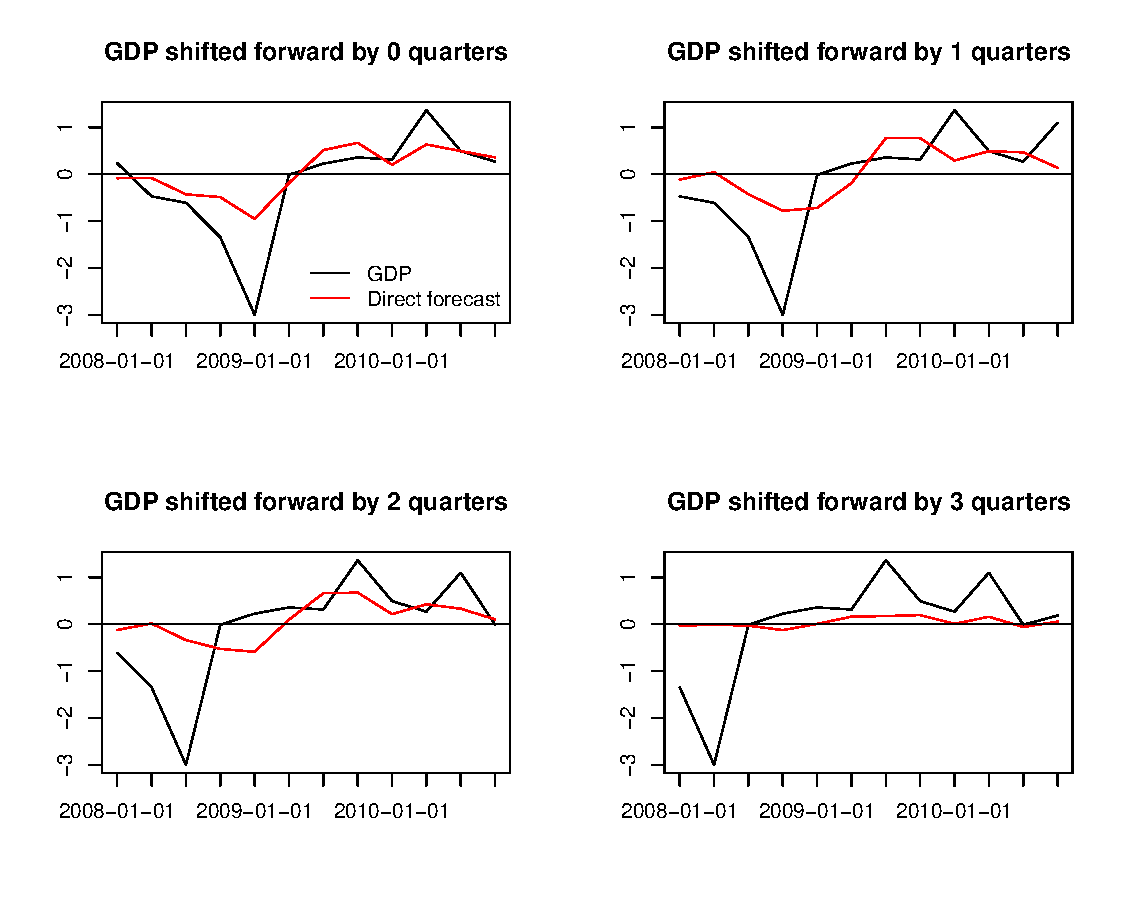
\includegraphics[width=0.9\textwidth]{./Figures/direct_wc_financial_crisis.pdf}
        \caption{Direct forecast across the financial crisis:  regression based on all indicators and full sample information, without pandemic.
        \label{direct_wc_financial_crisis}}
    \end{center}
\end{figure}

The results indicate that as the forecast horizon $h$ increases, the turning points (i.e., peaks and troughs) of the direct forecasts become increasingly right-shifted (lagged) relative to the target GDP. Additionally, the p-values of the HAC-adjusted Wald test precipitously increase from $h=2$ to $h=3$ (see Table \ref{tab:pvaluedhp}), implying that the indicators become statistically insignificant for forecast horizons of more than two quarters.\footnote{ 
These findings are confirmed by the relative root mean-square errors comparing direct forecasts against the mean benchmark, see Table \ref{rRMSE_mSSA_direct_mean_without_covid8} in the Appendix.} 

%\begin{table}[ht]
%\centering
%\begin{tabular}{rrrrrrrr}
%  \hline
% & h=0 & h=1 & h=2 & h=3 & h=4 & h=5 & h=6 \\ 
%  \hline
%P-values & 0.000 & 0.000 & 0.007 & 0.946 & 0.603 & 0.096 & 0.181 \\ 
%   \hline
%\end{tabular}
%\caption{Statistical significance of direct forecasts.  } 
%\label{tab:f_stats}
%\end{table}

\subsection{Direct Forecasts Based on Filtered Indicators}\label{hpdf}
%\subsection{Filter: HP(160)}

%As shown, the performance of direct forecasts sharply declines for longer forecast horizons. 
We conjecture that economic indicators may be contaminated by unpredictable high-frequency noise, thereby obscuring the effective `signal' and making a direct regression more susceptible to overfitting. If so, it may be possible to highlight the signal by filtering our indicators to dampen high-frequency noise. 

The Hodrick-Prescott (HP) filter is a classic tool used in business cycle analysis: the filter is specified by a single smoothing parameter $\lambda$ and the value $\lambda=1600$ is specifically recommended for quarterly data. However, \cite{Phillips_Jin_2021} noted that the HP(1600) filter removes relevant information due to excessive smoothing. In our context, this oversmoothing issue would be further exacerbated when considering forecast horizons shorter than a year---an interval inconsistent with the mean duration of up to several years of business cycles, as highlighted by the HP(1600). To address this concern, we suggest a more adaptive HP(160) `target' filter. 

Figure \ref{hp_160} presents both classic two-sided and one-sided HP(160) (denoted HP-C for \textit{concurrent}) filters (top panels) along with their associated amplitude functions in the frequency domain (bottom panels). It confirms that the HP-C filter assigns greater weight to yearly components—relevant in a mid-term forecast context— than the classic quarterly HP filter, while also reducing undesirable high-frequency noise. Therefore, while the choice of the HP(160) filter in this example
is somewhat arbitrary, it should serve the purpose of reducing high-frequency noise while preserving longer-duration movements.\footnote{A comprehensive technical analysis of the effect of $\lambda$ on the resulting GDP predictor can be conducted using the M-SSA package (\url{https://github.com/wiaidp/R-package-SSA-Predictor}).}

\begin{figure}[h]
    \begin{center}
        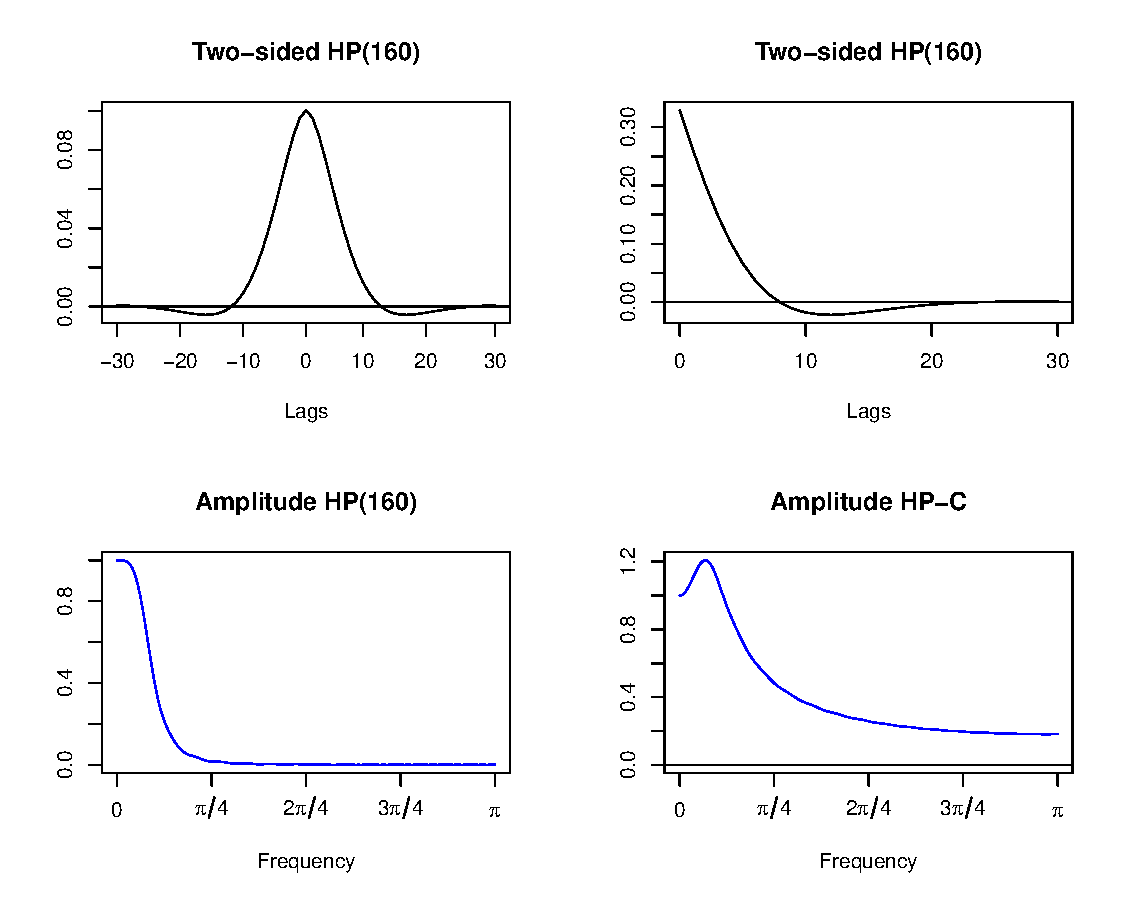
\includegraphics[height=4in, width=5.5in]{./Figures/hp_160.pdf}
        \caption{Two-sided HP(160) (top left) and one-sided (concurrent) HP-C filters (top right) with corresponding amplitude functions (bottom).
        \label{hp_160}}
    \end{center}
\end{figure}

%\subsection{Direct HP Forecast}\label{hpdf}

%Extending the `classic' direct forecast design, we consider filtered indicators, based on the one-sided HP(160), denoted as the HP-C filter: the filtered indicators are explanatory variables for the regressions on forward-shifted GDP. As in the previous section, we rely on all indicators as well as the full sample estimate for illustration, 

Figures \ref{direct_hp_forecasts} and \ref{direct_hp_forecasts_financial_crisis} provide results comparable to those of Figures \ref{direct_wc} and \ref{direct_wc_financial_crisis} but now using indicators smoothed with the HP-C filter, covering the full sample without the pandemic and providing a closer look at performance during the financial crisis.  The fitted values lag GDP slightly less and track turning points somewhat more quickly. Table \ref{tab:pvaluedhp} shows p-values for tests of the joint null hypothesis that all coefficients ${\boldsymbol{\beta}} = 0$. The use of filtered indicators improves their statistical significance at forecast horizons $h > 2$ quarters. 
%Figures \ref{direct_hp_forecasts} (all observations with exclusion of the pandemic) and \ref{direct_hp_forecasts_financial_crisis} (financial crisis). A comparison with the classic (unfiltered) direct forecasts in the latter figure %in Fig.\eqref{direct_wc_financial_crisis} 
% indicates that the new predictors are slightly less retarded and track the turning points more promptly (`faster'). 
% The filtered approach also exhibits superior statistical properties. As shown in Table \ref{tab:f_stats}, 
%The p-values of the F-statistics for the HP-based forecasts are smaller than for the direct forecasts specifically at $h=3$, but the predictor remains statistically insignificant at forecast horizons exceeding two quarters (even though the evaluation is conducted in-sample and based on all available indicators). 

\begin{figure}[H]
    \begin{center}
        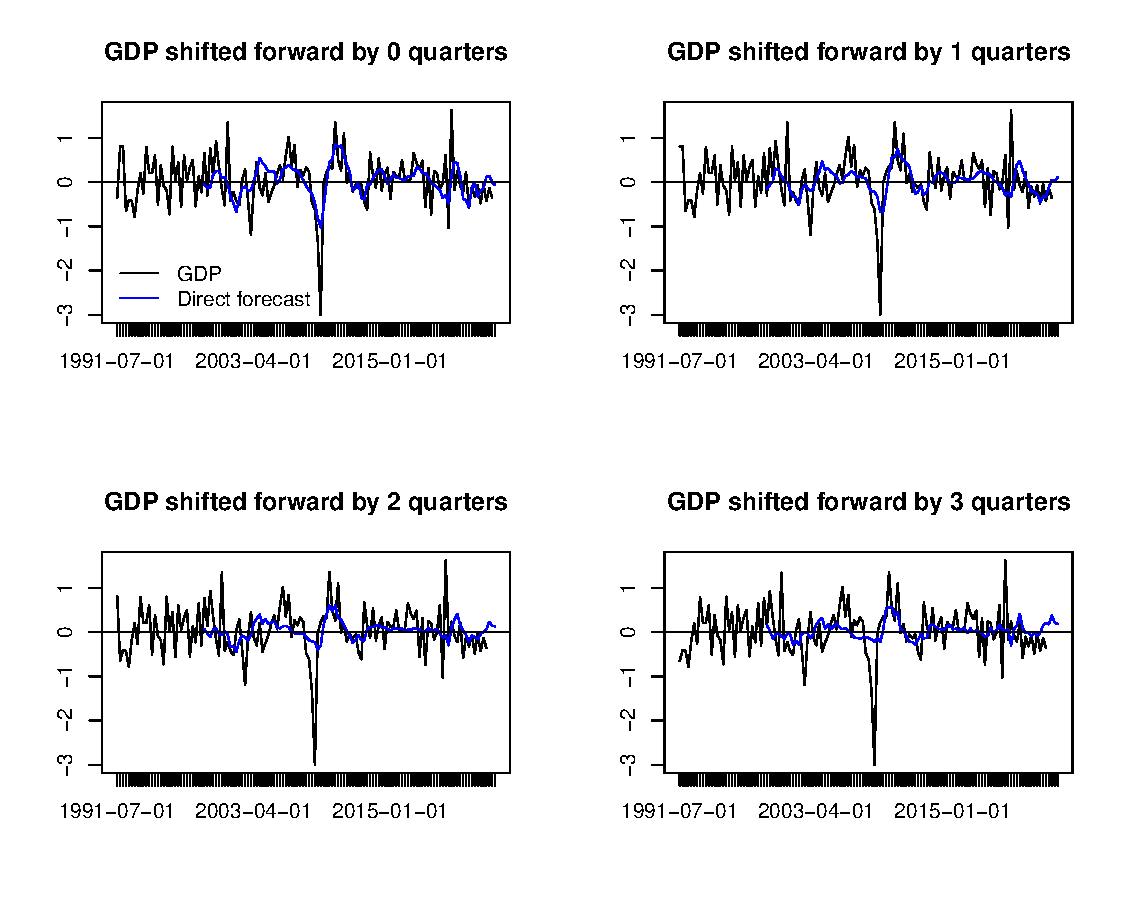
\includegraphics[width=0.85\textwidth]{./Figures/direct_hp_forecasts.pdf}
        \caption{Direct HP forecasts: entire data set with exclusion of the pandemic.
        \label{direct_hp_forecasts}}
    \end{center}
\end{figure}

\begin{figure}[H]
    \begin{center}
        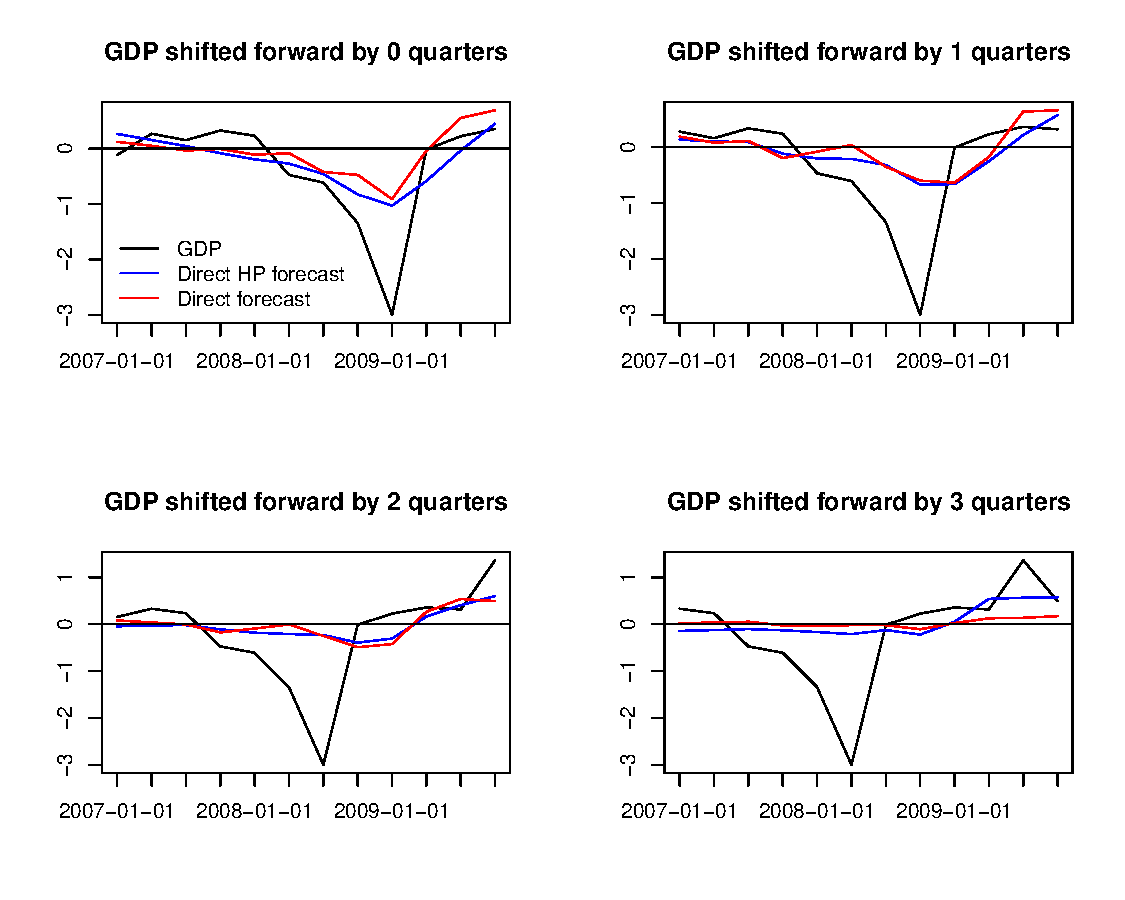
\includegraphics[height=5in, width=6in]{./Figures/direct_hp_forecasts_financial_crisis.pdf}
        \caption{Shifted GDP (black), direct HP forecast (red) and classic direct forecast (blue) over the course of the financial crisis: regression based on all indicators and full sample information (without pandemic).
        \label{direct_hp_forecasts_financial_crisis}}
    \end{center}
\end{figure}

% latex table generated in R 4.2.2 by xtable 1.8-4 package
% Wed May  7 12:49:46 2025

%\begin{table}[ht]
%\centering
%\begin{tabular}{rrrrr}
%  \hline
% & h=3 & h=4 & h=5 & h=6 \\ 
%  \hline
%rRMSE & 0.962 & 0.967 & 0.990 & 0.967 \\ 
%   \hline
%\end{tabular}
%\caption{Relative root mean-square error of HP-C against classic direct forecast for $h\geq %3$.\\Values $<1$ imply  HP-C has smaller RMSE.  } 
%\label{tab:rRMSE}
%\end{table}
\begin{table}[h]
\centering
\begin{tabular}{lrrrrrr}
  \hline
  & h= 1 & h= 2 & h= 3 & h= 4 & h= 5 & h= 6 \\ 
  \hline
  Unfiltered & 0.000 & 0.001 & 0.910 & 0.509 & 0.091 & 0.178 \\ 
HP-C filtered & 0.001 & 0.036 & 0.046 & 0.049 & 0.012 & 0.022 \\ 
   \hline
\end{tabular}
\caption{p-values for $H_0: \boldsymbol{\beta} = 0$, HAC-adjusted Wald test.\\Estimation over full sample (without pandemic.)} 
\label{tab:pvaluedhp}
\end{table}



%We now propose a more refined causal filter design aiming for statistical significance of the resulting predictor at longer forecast horizons, out-of-sample.   

\section{Multivariate Causal Filter: M-SSA}\label{sec:mSSA}

The application of the one-sided HP-C filter to the indicators yields some measurable improvements in forecast performance. However, its univariate nature excludes additional information such as that provided by leading indicators. The noise suppression capability of the one-sided filter is compromised, as explained by \cite{Wildi2025} and illustrated by the high-frequency leakage of the amplitude function in Figure \ref{hp_160}. To address these limitations, we propose an extension of the Smooth Sign Accuracy (SSA) framework introduced by \cite{Wildi2025}.

\subsection{Optimization criterion}

Let $\mathbf{X}_t$ (of dimension $t\times n$) denote a set of $n$ explanatory series $\mathbf{x}_{1t},...,\mathbf{x}_{nt}$, with observations $\mathbf{x}_{it}=(x_{i1},...,x_{it})'$. Let $\mathbf{z}_t=(z_{1},...,z_t)$  denote a target series, which typically lies outside the linear space spanned by $\mathbf{X}_t$  (and is unknown at time $t$). For simplicity, we assume stationarity of all time series involved. In this framework, $\mathbf{X}_t$ corresponds to a matrix of selected economic indicators with $n=5$, and $z_{it}$, i=1,...,5,   is the output of a two-sided HP(160) filter applied to the four indicators as well as to GDP. Since $z_{it}$  depends on future observations $x_{it+1},x_{it+2},...$, the prediction task involves `tracking' $z_{it}$  using the estimate $y^i_{t}=\sum_{j=1}^ny^i_{jt}$, where $y^i_{jt}=\mathbf{b}^i_j~'\mathbf{x}_{jt}=\sum_{k=0}^{L} b^i_{jk}x_{j,t-k}$ are the outputs of a multivariate (causal or one-sided) filter $\mathbf{B}^i$, with columns $\mathbf{b}^i_{j}$ of fixed length $L$, $j=1,...,5$, assigning weights to the last $L$ observations of the $j$-th indicator $\mathbf{x}_{jt}$ (the fixed-length assumption is merely used for ease of exposition).
For the sake of clarity, we now omit the index $i$ for all variables, assuming $z_t=z_{i_0t}$ for some fixed $i_0$.% Additionally, we assume a fixed filter length $L$, such that $\mathbf{B}^i_t=\mathbf{B}_t=\mathbf{B}$, which has dimension $L\times 5$. 

The task of `tracking' a target can be formalized in different ways; here, we focus on the correlation $\rho(z,y,h)$ between $y_t$ and target $z_{t+h}$, where $h\geq 0$ denotes the forecast horizon (backcasting with $h<0$ is ignored in this context). For simplicity, assume a fixed horizon, say $h=h_0$, so that we may drop the reference to $h$ in our notation. In the univariate case ($n=1$), \cite{Wildi2025} proposes the Smooth Sign Accuracy (SSA) as an optimization criterion:
\begin{eqnarray}\label{critssa}
\left.\begin{array}{c}\rho(z,y)\to\max\\
s.t. \quad \rho(y,1)=\rho_1\end{array}\right\}
\end{eqnarray}
where $\rho(y,1)$ is the first-order autocorrelation of the predictor $y_t$. The parameter $\rho_1$ controls the smoothness of the predictor: higher values of $\rho_1$ favour smoother trajectories of $y_t$. Assuming that the process $x_t$ has mean zero, \cite{Wildi2024} establishes a connection between $\rho(y,1)$ and the expected duration between consecutive `zero-crossings' (sign changes) of $y_t$, the `holding time', denoted by $HT(y)$\footnote{Formally, the precise relationship between the expected duration between sign changes and the lag-one autocorrelation of the predictor is derived under the assumption of Gaussian time series. However, \cite{Wildi2024} demonstrates that this relationship remains robust even when deviations from Gaussianity occur (central limit theorem applied to lowpass-filtered series).}:
\begin{eqnarray}\label{ht}
HT(y)=\frac{\pi}{\arccos(\rho(y,1))}.
\label{eq:ht_arccos}
\end{eqnarray}
Since eq. \ref{eq:ht_arccos} is strictly monotonic, the SSA criterion can be reformulated as the optimization problem:
\begin{eqnarray}\label{critssaht}
\left.\begin{array}{c}\rho(z,y)\to\max\\
\frac{\arccos(\rho(y,1))}{\pi}=1/HT_1\end{array}\right\},
\end{eqnarray}
where the smoothness parameter $1/HT_1$ expresses the expected rate of sign changes of the predictor. \\


Eq. \eqref{critssaht} has several important implications. First, the objective function is indifferent to an affine transformation of the predictor. This ambiguity can be resolved by assuming an arbitrary scale and level for $y_t$ (standardization). Alternatively, a mean square error norm (MSE) can be substituted for the target correlation, as noted in \cite{Wildi2025}. In this case, the classic MSE predictor $y_{t,MSE}$ is obtained as a solution to the SSA criterion by insertion of $1/HT_1:=1/HT_{MSE}$ in the constraint, where $HT_{MSE}$ represents the holding time of $y_{t,MSE}$. %If the MSE predictor is noisy, which is often the case in applications, one can select $HT_1>HT_{MSE}$  in the constraint to address the rate of noisy crossings or false alarms. 
Second, the concept can be extended to a multivariate framework, denoted M-SSA, by generalizing the correlation functions as detailed in \cite{Wildi2025}. 
%Lastly, sign changes in trend growth, represented by zero-crossings of the target $z_t$, are indicative of relevant changes in the trajectory of the economy, for example, at transitions between expansions and recessions. 
Lastly, when $z_t$ is GDP growth, sign changes are indicative of expansions and recessions.
Unfortunately, classic predictors often generate excessively many false (`noisy') sign changes due to high-frequency leakage, as discussed above.
%as illustrated by the amplitude function in Figure \eqref{hp_160} (bottom right panel) and further elaborated upon by \cite{Wildi2025}. 
 \cite{Wildi2025} shows that the SSA criterion helps control this phenomenon,  see Fig.\ref{mssa_msse_zc} for illustration. Using the dual formulation of the criterion \eqref{critssaht}, the author demonstrates that the SSA solution yields the lowest zero-crossing rate among all (linear) predictors with equivalent target correlation. Consequently, the subsequent analysis employs the M-SSA framework to construct a `smooth' predictor $y_t$ for forecasting $z_{t+h}$. In particular, it is shown that controlling the zero-crossing rate within the M-SSA framework has a quantifiable effect on the hit rate and false positive rate.
 
 
 %In a second stage, serving as a generalization and refinement of the univariate HP-C utilized in the direct HP forecast.


\subsection{Example: Out of sample M-MSE vs. M-SSA Nowcasts}

For illustration, consider the problem of nowcasting HP-filtered GDP, denoted by HP-GDP, where the target $z_t$ is generated using the two-sided HP(160) filter examined previously. We compare the classic multivariate mean squared error (MSE) predictor (denoted M-MSE) with the M-SSA predictor where we set $HT_1=1.5\times HT_{MSE}$. This constraint ensures that the M-SSA predictor produces roughly 33$\%$ fewer sign changes than M-MSE in large samples. Comparisons with M-MSE allow us to see the cost of this constraint in terms of prediction performance (target correlation). 
Both predictors use the same underlying VAR(1) model introduced in Section \ref{sec:direct_forecast} and estimated on data up to Q4-2007. This ensures a lengthy out-of-sample period that includes significant events such as the financial crisis, the sovereign debt crisis, and the COVID-19 pandemic.\footnote{The economic sentiment indicator (ESI) does not receive any weight in the parsimonious VAR(1) model estimated over the shorter sub-sample ending in Q4-2007. Technical details and background information on the M-SSA are provided in \cite{Wildi2025}. All computations are conducted using the M-SSA package, as documented in \cite{Wildi2025}. The package can be accessed at \url{https://github.com/wiaidp/R-package-SSA-Predictor}.}

\begin{figure}[htpb]
    \begin{center}
        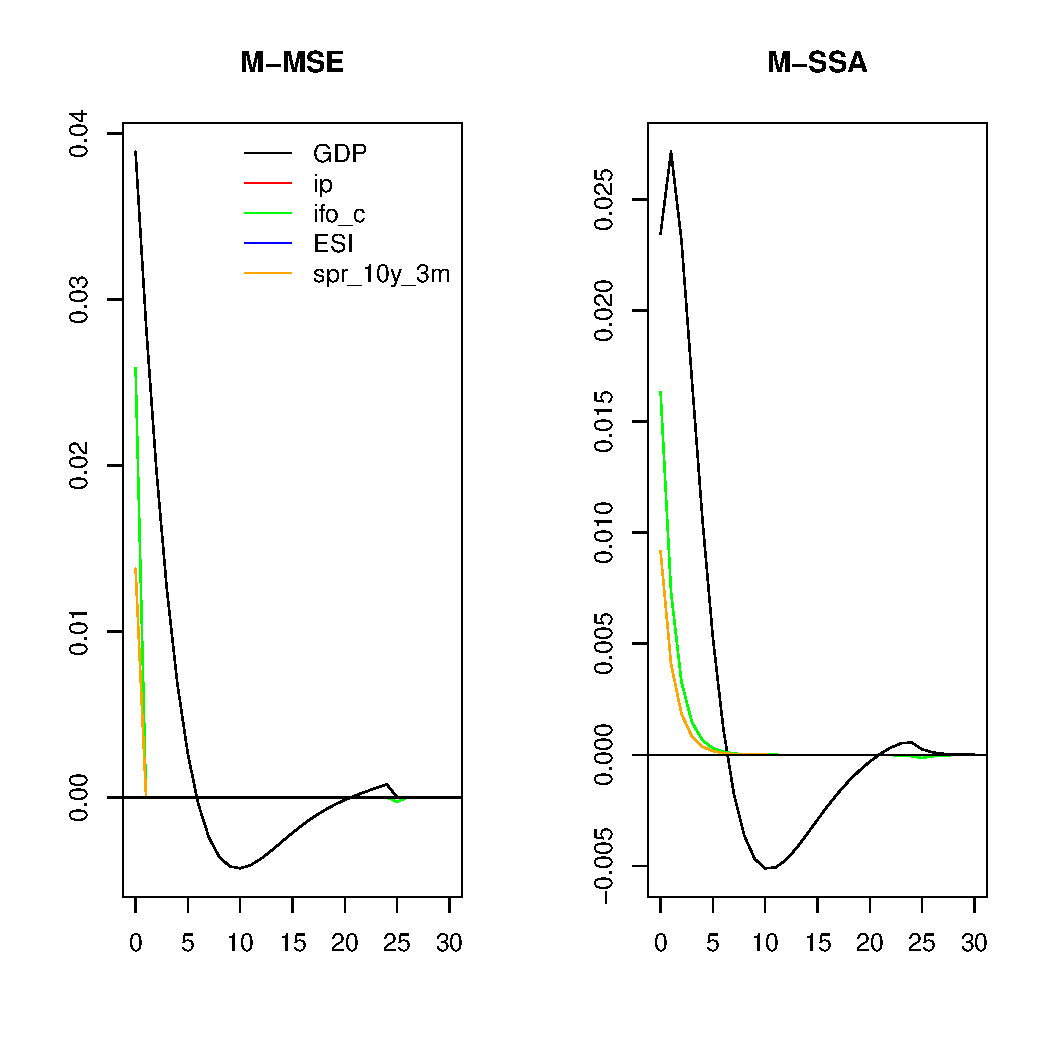
\includegraphics[height=3in, width=4.5in]{./Figures/bk_gammak.pdf}
        \caption{Multivariate M-MSE (left) and M-SSA (right) nowcast filter weights.
        \label{bk_gammak}}
    \end{center}
\end{figure}

\begin{figure}[htpb]
    \begin{center}
        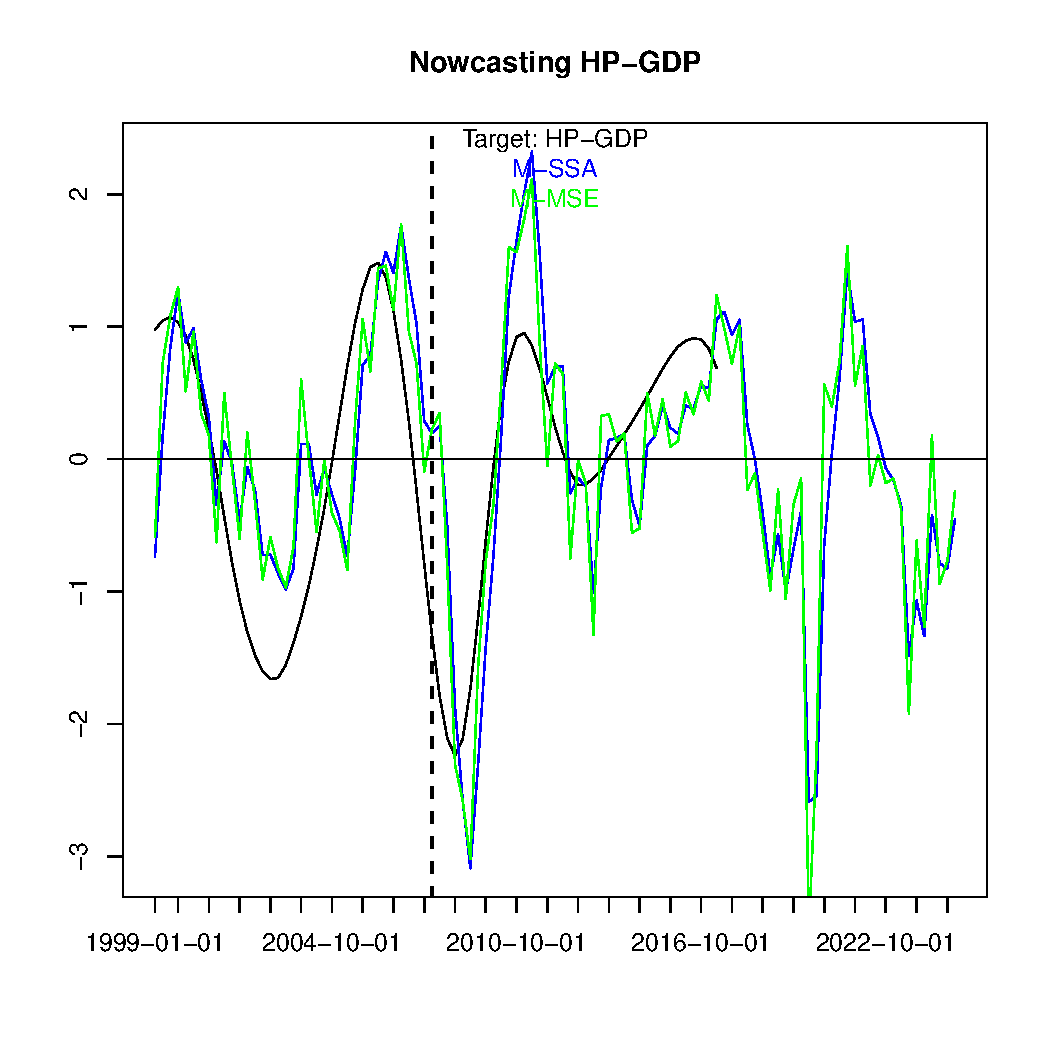
\includegraphics[height=3in, width=4.5in]{./Figures/mssa_msse_now.pdf}
        \caption{Two-sided HP(160) applied to GDP (black)\\ Nowcasts: M-SSA (blue) and M-MSE (green). \\The dashed vertical line delimits in- and out-of sample periods.  \\The two-sided filter does not extend to the sample end.
        \label{mssa_msse_now}}
    \end{center}
\end{figure}

\begin{figure}[H]\begin{center}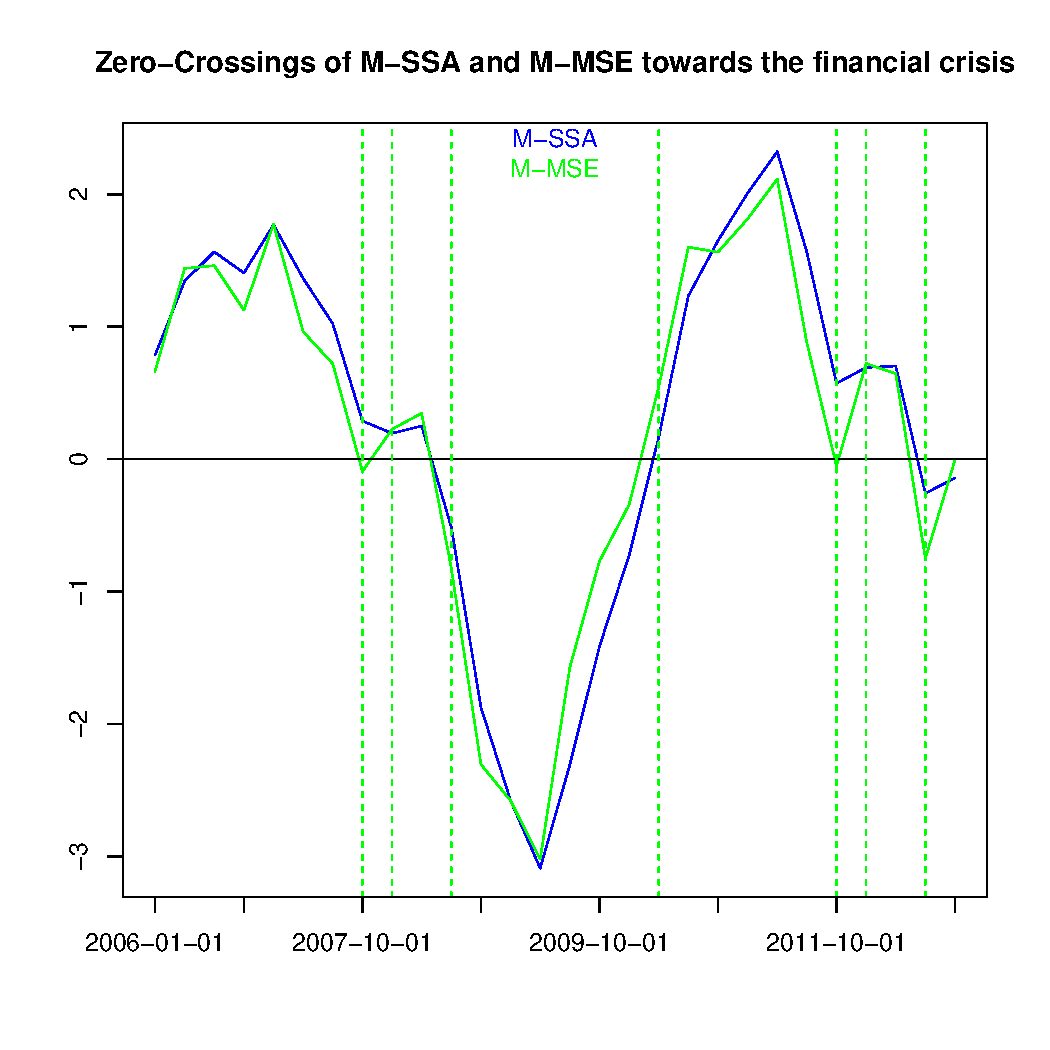
\includegraphics[height=3in, width=4.5in]{./Figures/mssa_msse_zc.pdf}\caption{Sign changes of the M-MSE (green) and M-SSA (blue) nowcasts towards the financial crisis, with sign changes of the M-MSE marked by green vertical lines. The sample holding time (HT) of each filter corresponds to the average duration between its consecutive zero-crossings. For each filter, its sample HT converges to the respective expected HT asymptotically. Here, we impose  $HT_{MSSA}=1.5\times HT_{MSE}$: in the long run, we expect the M-MSE to exhibit approximately $50\%$ more sign changes than the M-SSA.\label{mssa_msse_zc}}\end{center}\end{figure}
% latex table generated in R 4.2.2 by xtable 1.8-4 package
% Wed May  7 12:49:47 2025
\begin{table}[ht]
\centering
\begin{tabular}{lrr}
  \hline
 & M-SSA & M-MSE \\ 
  \hline
Target correlation & 0.68 & 0.69 \\ 
  HT & 6.50 & 3.71 \\ 
   \hline
\end{tabular}
\caption{Sample target correlations and holding times (HT) of M-SSA and M-MSE nowcasts.} 
\label{corhtnow}
\end{table}

Figure \ref{bk_gammak} displays the coefficients of the multivariate nowcasts, where M-SSA's increased smoothing reduces the maximum amplitudes of the filter weights and slows their rate of decay at longer lags. The resulting filtered series, presented in Figure \ref{mssa_msse_now}, are standardized to enable direct comparisons. The M-SSA nowcast is slightly smoother than that of the M-MSE, exhibiting approximately one-third fewer sign-changes. Fig.\ref{mssa_msse_zc} compares both nowcasts in relation to the financial crisis, highlighting that the classic (MSE-based) design tends to produce unwanted `noisy' zero-crossings at (or in the vicinity of) the transitions between recessions and expansions. Further, Table \ref{corhtnow} compares sample target correlations and HTs of the two nowcasts. Increased smoothness, i.e. holding time increases from 3.7 to 6.5 quarters, achieved by the M-SSA comes at the cost of a slight reduction (0.68 vs 0.69) in target correlation. This highlights the inherent trade-off—often referred to as the prediction dilemma—between smoothness (zero-crossing rate) and predictive accuracy (target correlation) within the M-SSA criterion. 
The results validate that the smoothing constraint incorporated into the multivariate extension of criterion \eqref{critssa} effectively manages the sign-changes of the predictor: sample estimates of the holding times align with the expected values derived from Eq.~\eqref{ht}.\footnote{Effective convergence of sample estimates to their theoretical expected values —assuming the true data-generating process is known— can be validated using the M-SSA package. This validation is typically performed through analyses of very long samples of simulated (multivariate) data, ensuring the consistency of the estimation procedures under idealized conditions.} An increase of $50\%$ in the HT relative to the M-MSE predictor has only a modest effect on the target correlation, suggesting that this trade-off could be beneficial in our application, as confirmed by a subsequent analysis of hit rate and false alarm rate. %Going forward, we now omit the M-MSE, as it is a special case of the more general M-SSA framework.


\subsection{Example: M-SSA Forecasts}

Next, we extend the previous example to consider forecasts of HP-GDP. The only modification this requires is to change $h=0$ (nowcast) to $h=1,...,6$ quarters. %The previously described nowcast example can be systematically extended to generate forecasts of the target variable. This extension utilizes the same empirical framework, incorporating an assumed $50\%$ increase in the HT over the M-MSE, and considers forward shifts of   (note that M-SSA does not target GDP explicitly). %This approach facilitates the assessment of forecast performance across multiple horizons within the established methodological context. 
The influence of the forecast horizon on the M-SSA design is depicted in Figure \ref{bk_h}, which contrasts M-SSA filter weights for the nowcast and the one-year-ahead forecast. Noting the difference in vertical scales, we see that as $h$ increases (right panel), the filter weights diminish, reflecting increased forecast uncertainty. We also see increased weight on the leading indicators relative to that on GDP.\footnote{Weights on IP and ESI are indistinguishable from zero.} Additionally, a phase shift associated with the filter applied to GDP is observed (black line, right panel), reflecting the cyclical characteristics inherent to the HP filter. While this phase effect might cause an effective sign change in the GDP filter output as $h$ increases—something to be avoided in this context—the low-pass filters assigned to the additional  `leading' indicators (green and yellow lines, right panel) continue to effectively track the low-frequency components of HP-GDP. The combination of the phase effect, applied to GDP, and level-tracking through these additional indicators enables more refined and effective tracking of the target compared to univariate forecasts, which rely solely on the phase-effect of the filter to look ahead.

\begin{figure}[H]
    \begin{center}
        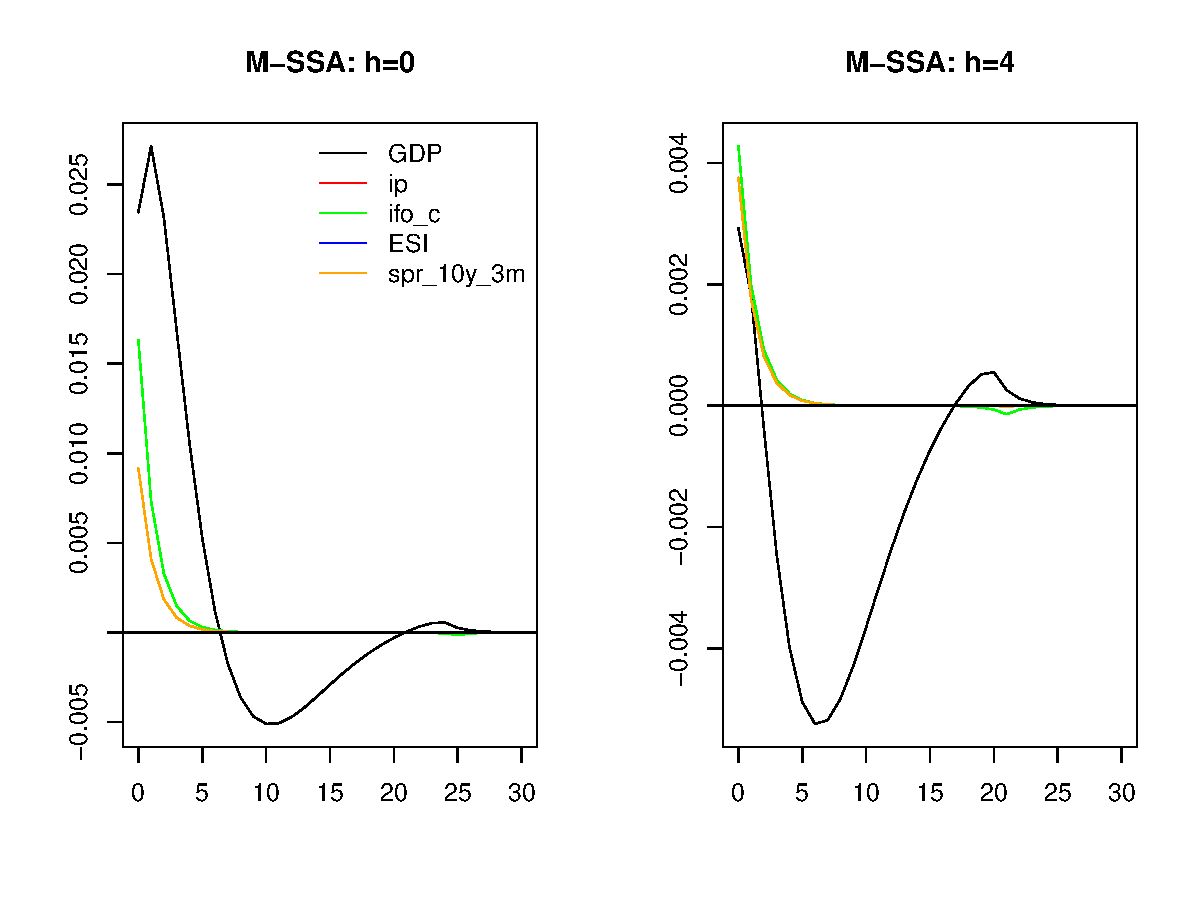
\includegraphics[width=0.85\textwidth]{./Figures/bk_h.pdf}
        \caption{Multivariate M-SSA filter weights: $h=0$ (nowcast, left) and $h=4$ (one year forecast, right).
        \label{bk_h}}
    \end{center}
\end{figure}

\begin{figure}[H]
    \begin{center}
        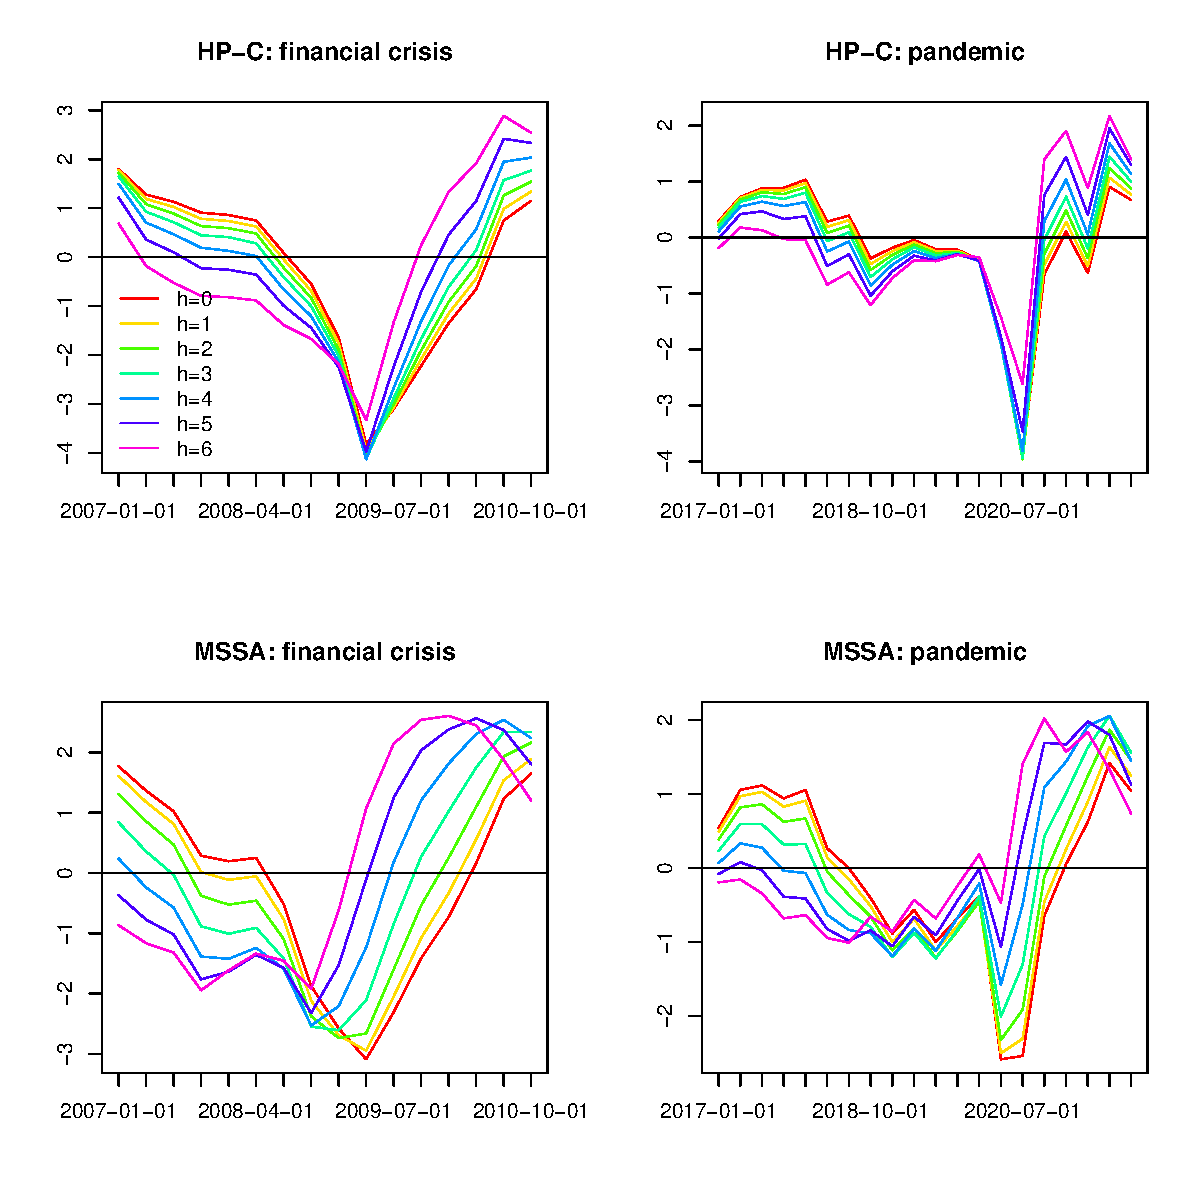
\includegraphics[width=0.85\textwidth]{./Figures/multivar_vs_univar.pdf}
        \caption{Now- and forecasts of HP-GDP for $h=0,...,6$: HP-C (top) vs. M-SSA (bottom) across the financial crisis (left) and the pandemic (right).
        \label{multivar_vs_univar}}
    \end{center}
\end{figure}


\begin{figure}[H]
    \begin{center}
        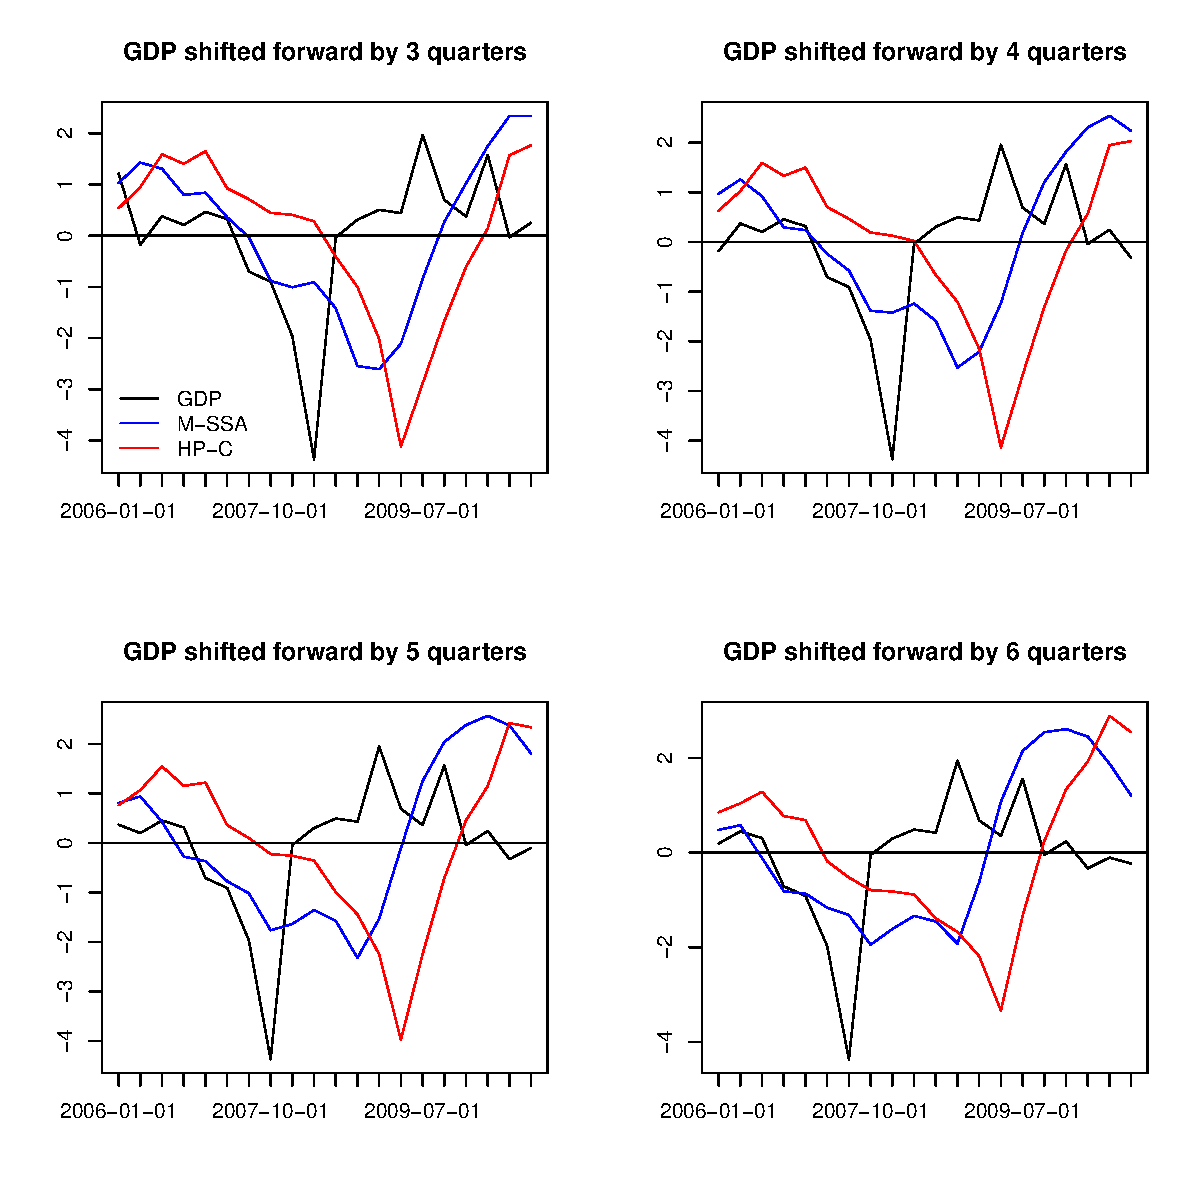
\includegraphics[width=0.85\textwidth]{./Figures/mssa_hpc_financial_crisis.pdf}
        \caption{Forward-shifted GDP (black), M-SSA (blue) and HP-C (red) for $h=3,4,5,6$ across the financial crisis. All series are standardized for ease of comparison.
        \label{mssa_hpc_financial_crisis}}
    \end{center}
\end{figure}




M-SSA predictors are compared to the traditional univariate HP-C in Figures  \ref{multivar_vs_univar} and \ref{mssa_hpc_financial_crisis}. In the first figure, we compare both filters across the periods of the financial crisis (top panels) and the COVID-19 pandemic (bottom panels), for forecast horizons $h=0,...,6$. 
%The nowcast from the previous section is included for reference. 
In the second figure, we compare both filters to the forward-shifted GDP for shifts larger than two quarters. All series are standardized for ease of comparison. Forecasts using the M-SSA approach consistently shift leftwards as $h$ increases; this shift appears to be consistent across all levels, including the peaks and troughs of the series. Conversely, the positions of peaks and troughs in the HP-C series are largely unaffected by increases in $h$. The leftward-shift of  the M-SSA forecasts can be partly attributed to the increasing weight assigned to the additional leading indicators, which dominate the GDP component at larger forecast horizons. %In comparison, the effect of phase shifts—arising from the cyclical nature of the HP-filter and manifesting in the HP-C forecasts (shown in the left panels)—seems less systematic. 
The systematic left-shift of the M-SSA is a key determinant of its out-of-sample forecast performances, as analyzed in the following section. 


\section{M-SSA Component Predictor}\label{sec:mSSA_component}

The targets of the multivariate filters above were the smoothed outputs obtained from the acausal two-sided HP(160) filter applied to the five indicators. However, our objective is to develop predictors for unfiltered GDP. To achieve this, we use the above M-SSA outputs $y_t^i, \: i = 1, \ldots, 5$ (referred to as M-SSA components) as predictors for forward-shifted GDP.
While we keep the M-SSA fixed, as based on data up to Q4-2007, we implement an expanding window starting from Q1-2008 for deriving the component weights, which are updated on a quarterly basis. 
%(this contrasts with Section \ref{sec:direct_forecast}, which was based on the full sample information). 
All the results that we present here exclude the pandemic; results including the pandemic are in the Appendix.\\


% \subsection{Standardized Predictor: Equal-Weighting}

% We begin with a simplifying assumption (relaxed in the next section) that all M-SSA components contribute equally to GDP prediction. This suggests averaging the standardized components to form an equally-weighted composite measure. Subsequently, the predictor is derived by regressing the (forward-shifted) GDP series on these standardized components. Figure \eqref{mssa_predictor} presents the GDP series alongside the equally-weighted M-SSA predictor. All series are standardized to facilitate visual comparison and to highlight the dynamic shifts, particularly the left-shift characteristic of the predictors.

% To enhance interpretability and assessment of the M-SSA predictor, we propose analyzing its individual components. For illustration, Figure \ref{mssa_predictor_interpretability} shows the nowcast at $h=0$. The solid blue line (the nowcast) approaches the zero line near the end of the sample, with a recent upward movement mainly supported by the leading spread component. In contrast, the ifo- and ESI-components remain near the zero line, while the ip- and GDP-components appear to be awaiting additional evidence and confirmation before signaling a definitive movement. This type of assessment can be useful for evaluating the relevance of recent changes in the forecasted time series dynamics.
% \begin{figure}[htpb]\begin{center}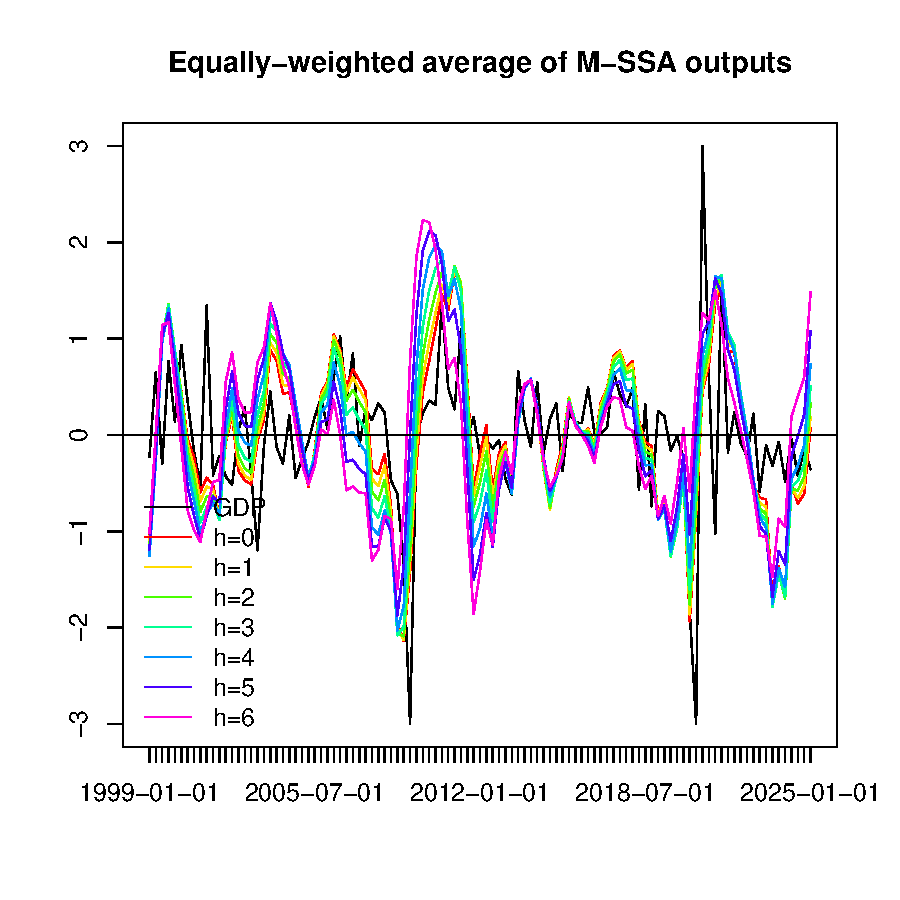
\includegraphics[height=3in, width=4.5in]{./Figures/mssa_predictor.pdf}\caption{GDP and equally-weighted M-SSA predictor: all series standardized.\label{mssa_predictor}}\end{center}\end{figure}\begin{figure}[htpb]\begin{center}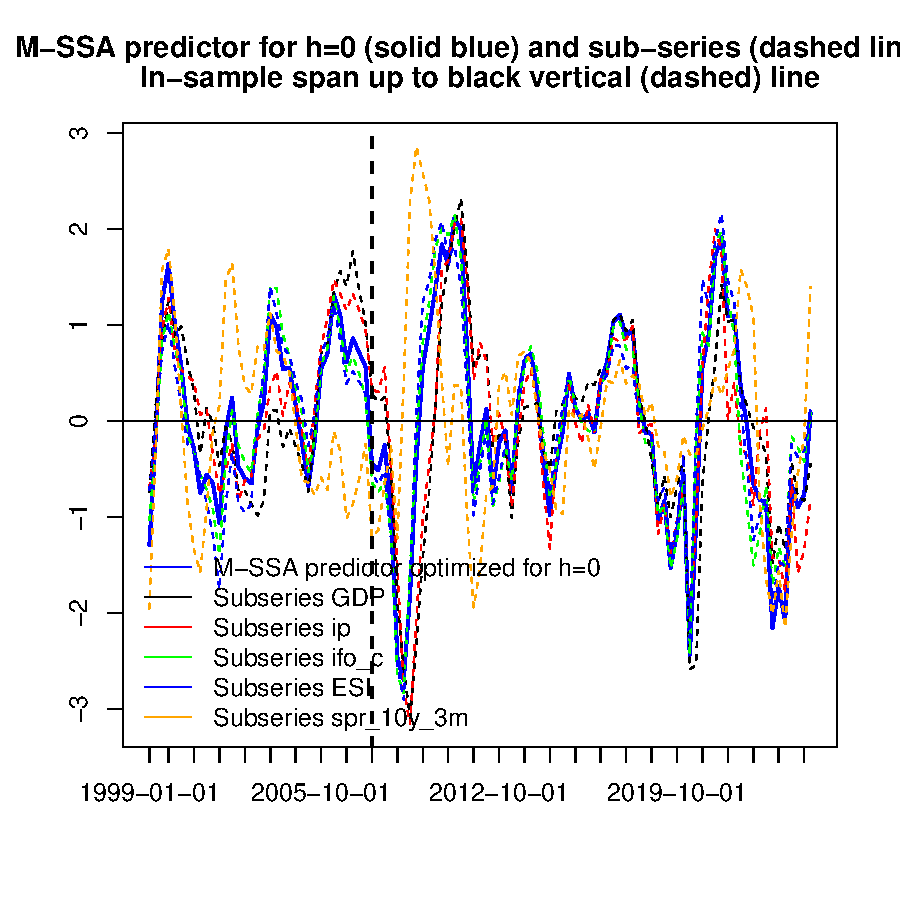
\includegraphics[height=3in, width=4.5in]{./Figures/mssa_predictor_interpretability.pdf}\caption{Equally-weighted M-SSA predictor and M-SSA components: all series standardized.\label{mssa_predictor_interpretability}}\end{center}\end{figure}

% \subsection{Tracking GDP: Optimal Weighting}


%We now utilize the M-SSA components as predictors for forward-shifted GDP.
%, extending the previous (standardized) equally-weighted M-SSA predictor to incorporate optimal weighting of the components. 


% There are various combinations of M-SSA components $y_t^i$ for tracking GDP. For illustration, we here select the single GDP component resulting from the M-SSA filter tracking HP-GDP
% \begin{equation}
%     \textrm{HP-GDP}_{t+shift}=\beta_0(shift,h)+\beta_1(shift,h)\cdot \textrm{M-SSA}^{\textrm{GDP}}_t(h) + \epsilon_t^{shift,h}
% \end{equation}

% In this expression, $\textrm{M-SSA}^{\textrm{GDP}}_t(h)$ is optimized for forecast horizon $h$, based on data up to January 2008. Table \eqref{p_val_hpbip_wc} reports HAC-adjusted p-values from regressions of the out-of-sample predictor on HP-GDP, indicating a strong link between the predictor and the target, out-of-sample. 
% % latex table generated in R 4.2.2 by xtable 1.8-4 package
% % Wed May  7 12:49:50 2025
% \begin{table}[ht]
% \centering
% \begin{tabular}{rrrrrrrr}
%   \hline
%  & h=0 & h=1 & h=2 & h=3 & h=4 & h=5 & h=6 \\ 
%   \hline
% Shift=0 & 0.000 & 0.000 & 0.001 & 0.002 & 0.005 & 0.020 & 0.112 \\ 
%   Shift=1 & 0.000 & 0.000 & 0.000 & 0.001 & 0.002 & 0.005 & 0.019 \\ 
%   Shift=2 & 0.000 & 0.000 & 0.000 & 0.001 & 0.001 & 0.003 & 0.006 \\ 
%   Shift=3 & 0.018 & 0.007 & 0.002 & 0.000 & 0.002 & 0.003 & 0.004 \\ 
%   Shift=4 & 0.180 & 0.100 & 0.040 & 0.010 & 0.002 & 0.005 & 0.005 \\ 
%   Shift=5 & 0.579 & 0.432 & 0.261 & 0.108 & 0.027 & 0.008 & 0.009 \\ 
%    \hline
% \end{tabular}
% \caption{Regression of shifted HP-GDP on M-SSA($h$) GDP component\\p-values for $H_0: \hat{\beta} = 0$, HAC-adjusted Wald test\\Out-of-sample evaluation starting in Jan-2007, without pandemic.} 
% \label{p_val_hpbip_wc}
% \end{table}Our choice—focusing on the single M-SSA GDP component—emphasizes simplicity and interpretability, as future GDP and HP-GDP are connected through their shared low-frequency component. Additionally, the M-SSA GDP component is the most important predictor in the regression of the M-SSA outputs on GDP.  Finally, revisions due to quarterly updates of the regression equations are minimized by this predictor, and the estimates are more stable and robust over time\footnote{Other combinations can be experimented with using the M-SSA package. Regression weights of more complex designs, involving multiple components, tend to be more difficult to interpret due to the occurrence of negative weights and potential sign changes of the regressors over time, which may indicate overfitting or non-stationarity.} (see Section \eqref{sec:revisions}). Note that information from the other indicators is incorporated into the M-SSA GDP component through the multivariate filter design.\\



% This setup allows us to evaluate the out-of-sample performance of various predictor approaches, including: (i) the simple mean of GDP, (ii) the direct forecast method described in Section \eqref{cdf}, (iii) the direct HP forecasts from Section \eqref{hpdf}, based on the univariate HP-C, and (iv) the new M-SSA GDP component predictor. %For completeness, we also consider an M-MSE component predictor derived from outputs of the multivariate MSE filter. 




%Out-of-sample performance metrics include p-values derived from regressions of the out-of-sample predictors on forward-shifted GDP, adjusted for heteroscedasticity and autocorrelation using HAC estimators. Additionally, we report relative root-mean-square forecast errors (rRMSE) benchmarked against various reference models.\\ 

\subsection{Tracking GDP: Optimal Weighting}

Let $\textrm{M-SSA}^{\textrm{GDP}}_t(h)$ denote the M-SSA predictor of HP-GDP for forecast horizon $h$. A predictor of GDP can be obtained from the simple regression equation
\begin{equation}
\textrm{GDP}_{t+shift}=\beta_0(shift,h)+\beta_1(shift,h) \cdot \textrm{M-SSA}^{\textrm{GDP}}_t(h) + \epsilon_t^{shift,h}
\label{eq:GDP_M-SSA}
\end{equation}
The purposes of the regression are twofold: first, the parameters enable affine transformations of the left-hand side variable, so that the standardized target $\textrm{GDP}_{t+shift}$ can be replaced by the original log-returns of GDP; second, the scale adjustment by $\beta_1(shift,h)$ compensates for the deflation (zero-shrinkage) of $\textrm{M-SSA}^{\textrm{GDP}}_t(h)$, reflecting greater uncertainty  as the forecast horizon $h$ extends. This simple transformation allows $\textrm{M-SSA}^{\textrm{GDP}}_t(h)$ to serve as a predictor for $\textrm{GDP}_{t+shift}$ even when $h\neq shift$. This flexibility enables leveraging the dynamic left-shift of $\textrm{M-SSA}^{\textrm{GDP}}_t(h)$, illustrated in Figure \ref{multivar_vs_univar}, when $shift<h$.\\

Define the (out-of-sample) GDP component predictor $\hat{\textrm{GDP}}_{t+shift}(h)$:  
\begin{equation}\label{oos_pred}
\hat{\textrm{GDP}}_{t+shift}(h):=\hat{\beta}_0(shift,h,t)+\hat{\beta}_1(shift,h,t) \cdot \textrm{M-SSA}^{\textrm{GDP}}_t(h),
\end{equation}
where the regression parameters $\hat{\beta}_0(shift,h,t),\hat{\beta}_1(shift,h,t)$ are estimated using data up to time point $t-1$ (expanding window). Since M-SSA is based on data up to Q4-2007, $\hat{\textrm{GDP}}_{t+shift}(h)$ constitutes an out-of-sample predictor of $\textrm{GDP}_{t+shift}$ for all positive $shift\geq 0$ and all $t$ larger than Q4-2007. Define the out-of-sample forecast error
\begin{equation}\label{oosfe}
\hat{\epsilon}_t^{shift,h}:={\textrm{GDP}}_{t+shift}-\hat{\textrm{GDP}}_{t+shift}(h).
\end{equation}
We now assume that the regression parameters $\hat{\beta}_0(shift,h,t)$ and$,\hat{\beta}_1(shift,h,t)$ in Equation \ref{oos_pred} are up-dated quarterly. Note that Equations \ref{eq:GDP_M-SSA} and \ref{oos_pred} could be extended to incorporate additional M-SSA components, but for illustration purposes, we focus on the simplest (and most robust) design.


\subsection{Out-of-Sample Forecast Performances}\label{oosp}

The statistical significance of the (out of sample) GDP component predictor in Equation \ref{oos_pred}  can be evaluated by regressing 
$\textrm{GDP}_{t+shift}$ on $\hat{\textrm{GDP}}_{t+shift}(h)$:
\begin{equation}\label{eq_gdp_pred}
\textrm{GDP}_{t+shift}=\alpha_0+\alpha_1\hat{\textrm{GDP}}_{t+shift}(h)+\nu_{t}^{shift,h},
\end{equation}
for observations after Q4-2007: the significance of the corresponding HAC-adjusted statistics is indicated by a `star' symbol in Table \ref{rRMSE_mSSA_comp_mean_wc}\footnote{A single star means significance at the $5\%$ level; a double star means significance at the $0.1\%$ level. Note that statistical significance is influenced by the relatively short out-of-sample span, of length 17 years.}. The MSE forecast performance of $\hat{\textrm{GDP}}_{t+shift}(h)$ can be benchmarked against the mean predictor (see Table \ref{rRMSE_mSSA_comp_mean_wc} which reports relative Root Mean-Square Errors, rRMSE) as well as against the direct forecast (see Table \ref{rRMSE_mSSA_comp_direct_without_covid7}). For consistency, both benchmark predictors are also quarterly updated out-of-sample designs.\\

% Obviously, predicting HP-GDP (see Table \ref{p_val_hpbip_wc}) is less challenging than predicting GDP (see Table \eqref{p_val_wc}), due to smoothness (autocorrelation) of the target when compared to GDP. 

Our results can be summarized as follows. When excluding the pandemic, the direct forecasts outperform the mean forecast up to two quarters ahead, see Table \ref{rRMSE_mSSA_direct_mean_without_covid8} in the appendix. %\footnote{However, the pandemic period generally obscures the relationships between predictors and GDP.}.
In contrast, the GDP component predictors $\hat{\textrm{GDP}}_{t+shift}(h)$, optimized for longer forecast horizons $h\geq 5$, outperform the mean benchmark up to 5Q ahead, see Table \ref{rRMSE_mSSA_comp_mean_wc}. Additionally,  $\hat{\textrm{GDP}}_{t+shift}(h)$, optimized for large forecast horizons $h\geq 4$, surpass the direct forecasts for $shift\geq 3$, see Table \ref{rRMSE_mSSA_comp_direct_without_covid7} in the appendix. Statistical significance of the GDP component predictor, optimized for larger forecast horizons, can be established for at least up to one year ahead, see Table \ref{rRMSE_mSSA_comp_mean_wc}. Finally, the strong performance of predictors optimized for larger forecast horizons ($h\geq 4$), at smaller shifts ($shifts< 4$) corroborates the importance of the left-shift of the corresponding predictors, see Figs.\ref{multivar_vs_univar} and \ref{mssa_hpc_financial_crisis}, in relation to forecast performance.  


%???check whether rMSE is decreasing towards sample end (because initial estimate towards 2007 is unreliable)???


\begin{table}[ht]
\centering
\begin{tabular}{rrrrrrrr}
  \hline
 & h=0 & h=1 & h=2 & h=3 & h=4 & h=5 & h=6 \\ 
  \hline
Shift=0 & 0.975 & 0.941^{*} & 0.886^{*} & 0.839^{**} & 0.843^{**} & 0.897^{**} & 0.965 \\ 
  Shift=1 & 1.085 & 1.068 & 1.011 & 0.927^{*} & 0.871^{**} & 0.875^{**} & 0.919^{**} \\ 
  Shift=2 & 1.076 & 1.089 & 1.074 & 1.011 & 0.938^{*} & 0.902^{**} & 0.909^{**} \\ 
  Shift=3 & 1.037 & 1.069 & 1.090 & 1.059 & 0.992 & 0.943^* & 0.930^* \\ 
  Shift=4 & 1.013 & 1.058 & 1.101 & 1.097 & 1.037 & 0.967 & 0.925^* \\ 
  Shift=5 & 1.016 & 1.062 & 1.106 & 1.115 & 1.078 & 1.015 & 0.955^* \\  
   \hline
\end{tabular}
\caption{rRMSEs: out-of-sample forecast errors Equation \ref{oosfe} vs expanding mean of GDP\\Out-of-sample evaluation starting in Q1-2008, without pandemic\\Values $< 1$ indicate superior predictions from Equation \ref{oos_pred}\\
Row-index: Shift refers to the left-shift of the target $\textrm{GDP}_{t+shift}$\\
Column-index: $h$ refers to the forecast horizon for which $\textrm{M-SSA}_t^{\textrm{GDP}}(h)$ is optimized\\
Significance refers to the hypothesis $\alpha_1=0$ in Equation \ref{eq_gdp_pred}.
} 
\label{rRMSE_mSSA_comp_mean_wc}
\end{table}





\subsection{Hit Rate vs. False Alarm Rate}

To this point, indicators have been assessed by the extent to which they correlate with or lead movements in the target variable. An alternative approach would to be consider their ability to predict the correct ``type'' of outcome, e.g. whether growth will be stronger or weaker than average, or whether the economy will be in an expansion or a recession. 
This may be of particular interest to policymakers whose primary concern is to intervene ``in the right direction'' so as to stabilize the economy overall. We therefore limit our analysis to binary classifiers, focussing in particular on the ROC curve and the AUC.\footnote{For example, see \cite{YangLahiriPagan2024ROC} for a recent discussion of the ROC, the AUC and their relation to selected other binary classifiers. The discussion below follows their notation.}

Consider a binary random variable $Z \in \{0,1\}$ as our target, and a continuous variable $Y$. Our predictor for $Z$ is given by the function 

\begin{equation}
    \mathbf{1}(Y \leq \tau) \equiv I(\tau)
\end{equation}

where $\mathbf{1}()$ is the indicator function.\footnote{The value of the indicator function is equal to 1 when the condition in its argument is satisfied; otherwise the value of the function is equal to 0.}

The joint distribution of $Z$ and $Y$ allows us to define the Hit Rate $H(\tau)$ and the False Alarm Rate $F(\tau)$ as 

\begin{align}
    H(\tau) &\equiv Pr( Y \leq \tau | Z = 1)\\
    F(\tau) &\equiv Pr( Y \leq \tau | Z = 0)
\end{align}

The usefulness of a given variable $Y$ as a predictor will obviously depend on the value of $\tau$ selected, which in turn may be influenced by the relative importance attached to $H(\tau)$ and $F(\tau)$. To compare the range of possibilities associated with various choices for $Y$, we may plot on the unit square $F(\tau)$ vs $H(\tau)$ for all values of $\tau$ in the range of $Y$. This is called the Receiver Operating Characteristic (ROC) curve.

An ideal predictor would be one where $H(\tau) = 1$ and $F(\tau) = 0 \; \forall \tau $ (i.e. $Y > \tau$ whenever $Z=0$ and $Y \leq \tau$ whenever $Z=1$.) In this ideal case, the ROC curve would consist of the extreme left and top edges of the plot. Another extreme case would be one where $\{Y,Z\}$ are independent, so $H(\tau) = F(\tau) \; \forall \tau$. In this case, the ROC curve would simply be the 45-degree line through the origin. When comparing two indicators $Y_a$ and $Y_b$, if the ROC curve of $Y_a$ lies strictly above and to the left of that of $Y_b$, then we would always prefer to use $Y_a$ as our predictor in place of $Y_b$ since for any choice of $\tau$ it will always give us a superior trade-off between $H(\tau)$ and $F(\tau)$. When the ROC curves for two indicators cross, however, then our preferred indicator will depend on the relative importance that we attach to the hit and false alarm rates.\footnote{As shown in Wildi (2025), the sign accuracy can be related to the target correlation in the objective function of the (M-)SSA criterion; additionally, the rate of false alarms depends on the holding time (HT), so that the tradeoff underlying the ROC curve is to some extent captured by the M-SSA criterion.} 

A popular approximate measure of the overall performance of an indicator $Y$ that abstracts from the choice of $\tau$ is the Area Under the ROC Curve (AUC). Because the ROC is defined on the unit square, the maximum value of the AUC = 1. Above we saw that when $\{Y,Z\}$ are independent, the ROC curve lies on the 45-degree line, so the area under the curve is then 0.5. The range of AUCs between 1 and 0.5 therefore provides some quantitative guidance as to which predictor variables $Y$ have the potential to improve the prediction of $Z$.\footnote{AUCs $< 0.5$ suggest that $-Y$ may give more useful predictions than $Y$.}. 

%As shown in Wildi (2025), the SSA criterion's objective function—the target correlation $\rho(y,z,h)$—can be linked to the sign accuracy of the predictor $SA(y_t):=\text{P}\left(\text{sign}(z_{t+h}) = \text{sign}(y_t)\right)$, i.e., the probability that the signs of the predictor $y_t$ and the target $z_{t+h}$ agree:
%\begin{eqnarray}\label{sig_acc}
%SA(y_t)=0.5+\frac{\arcsin(\rho(y,z,h))}{\pi}.
%\end{eqnarray}
%Due to the strict monotonicity of the arcsin function, maximizing the target correlation also maximizes the sign accuracy of the predictor.\footnote{Equation \ref{sig_acc} holds exactly for Gaussian processes. Due to the central limit theorem, the relationship holds approximately for low-pass filtered non-Gaussian series, see Wildi (2025).} 


ROC curves are generated by evaluating the relationship between the sign of the target variable $GDP_{t+shift}$  and events where the forecast $\hat{GDP}_{t+shift}(h)$ exceeds a threshold $\tau$. The threshold $\tau$ is varied smoothly across the range of the predictor space to construct the ROC curve.\footnote{Although we are using standardized GDP, the regressions automatically account for scales and level shifts, so the results directly apply to the original GDP.} We examined all pairwise combinations of $h$ and $shift$, but for simplicity of exposition, the results below focus on the diagonal case where $h=shift$. 
For clarity, these results are based on the entire sample, excluding the pandemic period. Fig.\ref{ROC_GDP_shift_1_4} compares ROCs of the predictors for small and mid-term forecast horizons and Table \ref{auc} presents AUC (area under the curve) for forecast horizons 1-5 quarters ahead.
\begin{figure}[h]\begin{center}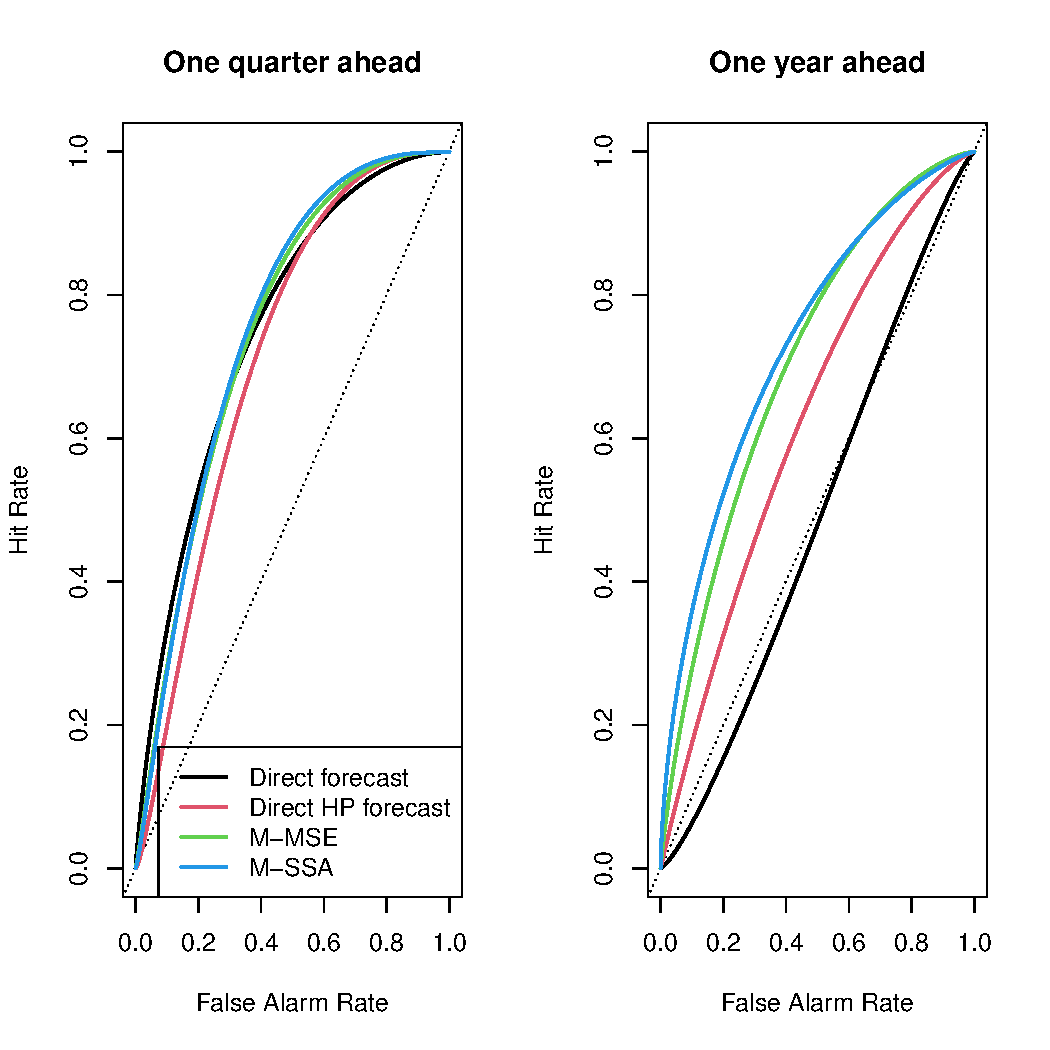
\includegraphics[height=3in, width=5in]{./Figures/ROC_GDP_shift_1_4.pdf}\caption{Hit rate vs. false alarm rate of the predictors at small (one quarter ahead:left panel) and yearly forecast horizons (right panel).\label{ROC_GDP_shift_1_4}}\end{center}\end{figure}
% latex table generated in R 4.2.2 by xtable 1.8-4 package
% Wed May 21 10:06:12 2025
\begin{table}[ht]
\centering
\begin{tabular}{rrrrr}
  \hline
 & Direct forecast & Direct HP forecast & M-MSE & M-SSA \\ 
  \hline
Forecast horizon 1 & 0.752 & 0.715 & 0.750 & 0.756 \\ 
  Forecast horizon 2 & 0.697 & 0.663 & 0.714 & 0.744 \\ 
  Forecast horizon 3 & 0.554 & 0.622 & 0.666 & 0.716 \\ 
  Forecast horizon 4 & 0.486 & 0.624 & 0.707 & 0.732 \\ 
  Forecast horizon 5 & 0.593 & 0.636 & 0.660 & 0.713 \\ 
   \hline
\end{tabular}
\caption{AUCs of predictors against GDP at various forecast horizons.} 
\label{auc}
\end{table}At forecast horizons less than or equal to two quarters, the direct forecast challenges the filters. However, for horizons $h>2$, the filters outperform the direct approach: the univariate HP-C design is surpassed by the classic multivariate MSE filter, which is in turn dominated by the M-SSA. These results confirm that controlling the rate of sign changes of the predictor, while maximizing its target correlation through M-SSA can enhance predictor performance in terms of sign accuracy and false alarm rate.



\section{Revisions}\label{sec:revisions}



Revisions refer to changes in the historical values of a time series resulting from updates with new information. Revisions of the M-SSA component predictor can arise from data updates, which we do not analyze further here\footnote{Except for GDP, the other indicators are not or only slightly revised. Moreover, the smoothing effect of filters mitigates the effect of revisions when compared to direct forecasts.}, or from updates to predictor parameters. The latter can be further separated into changes in the regression weights and VAR parameters. 


\subsection{Revisions: Regression Equation Only}

\begin{figure}[h]
    \begin{center}
        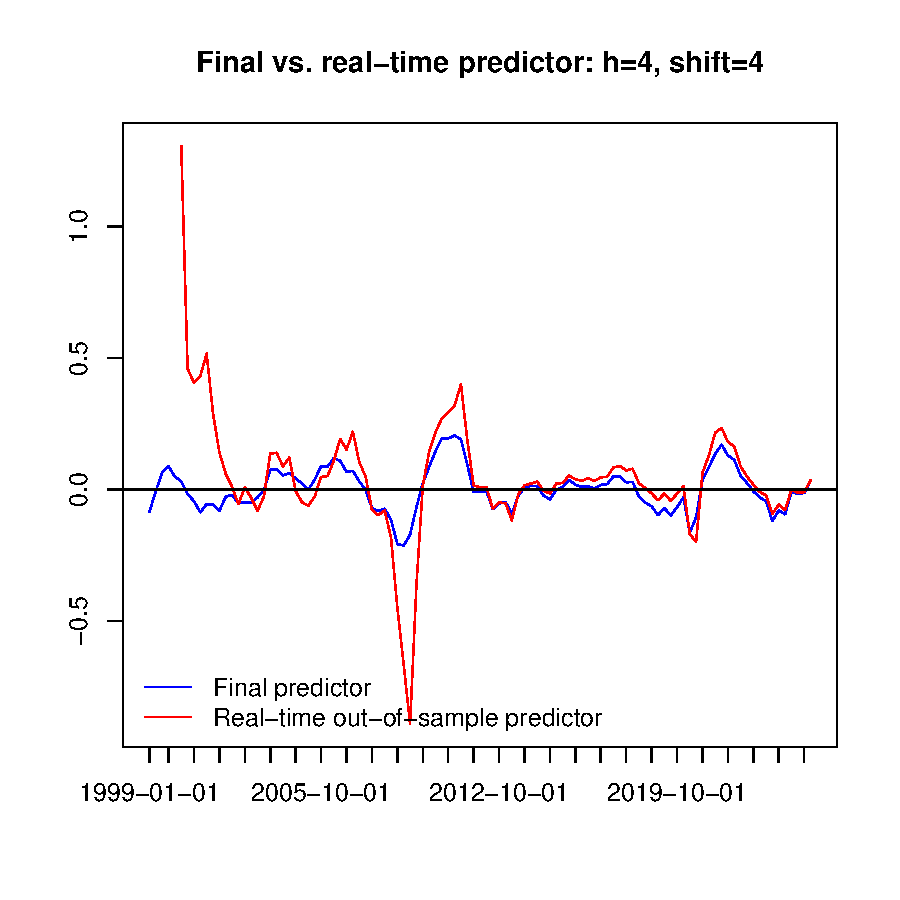
\includegraphics[height=3in, width=4.5in]{./Figures/revisions1.pdf}
        \caption{Revisions of the M-SSA GDP component predictor are shown, with the final predictor in blue and the real-time design in red. These revisions result from quarterly updates to the regression coefficients of equation \ref{oos_pred}. The M-SSA filter    itself remains fixed, based on data up to Q4-2007.
        \label{revisions1}}
    \end{center}
    \end{figure}

\begin{figure}[h!]
    \begin{center}
        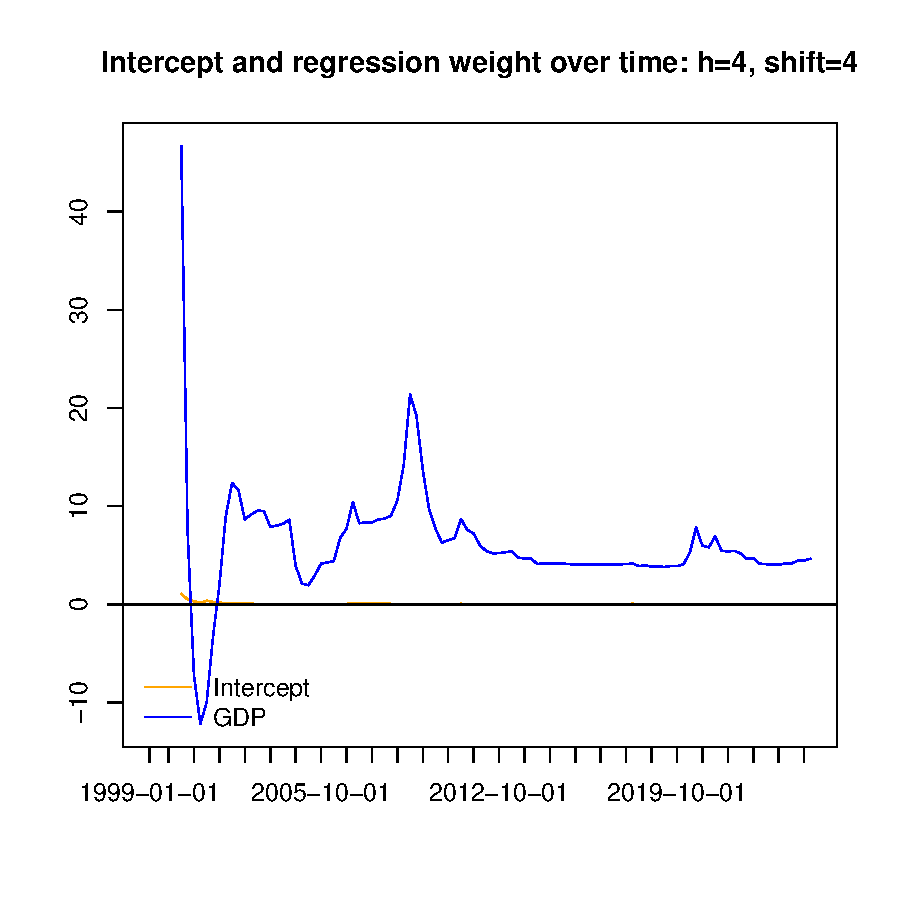
\includegraphics[height=3in, width=4.5in]{./Figures/revisions2.pdf}
        \caption{Revisions of intercept and regression weight of Equation \ref{oos_pred}.
        \label{revisions2}}
    \end{center}
\end{figure}

For illustration, we focus on a forecast horizon $h=4$ for the GDP component predictor and a forward-shift $shift=4$ for GDP, noting that similar results would be obtained with other combinations of $h$ and $shift$. 
%???Check left-shift of MA-inversion of M-SSA and M-MSE
%??? Check forecast excess for HP-C
%??? Justification HP(160): replace HP(1600) by AR(2) with similar persistency but shorter cycle lengthi, i.e. $a_1=-2"persistency*acos(\theta, a_2=persistency$.
Figure \ref{revisions1} compares the final and real-time predictors: as the sample size increases, the real-time predictor converges steadily to the final predictor.\footnote{The rate of convergence is partially determined by the simplicity of our design, which avoids incorporating additional M-SSA components.} 
As a confirmation, Figure \ref{revisions2} displays the evolution of the intercept and regression weights over time: with increasing sample size, these estimates seem to converge to fixed points, indicating both the stationarity of the process and the consistency of the estimates. %(Note, however, the slightly elevated values of the regression weight assigned to the M-SSA component during the financial crisis and the pandemic, suggesting a stronger link between the target and the predictor). 
In contrast, more complex designs based on multiple M-SSA components can exhibit substantial fluctuations in the regression parameters, sometimes changing signs. This suggests instability and complicates interpretation.

\subsection{Revisions: M-SSA Only}


\begin{figure}[h!]
    \begin{center}
        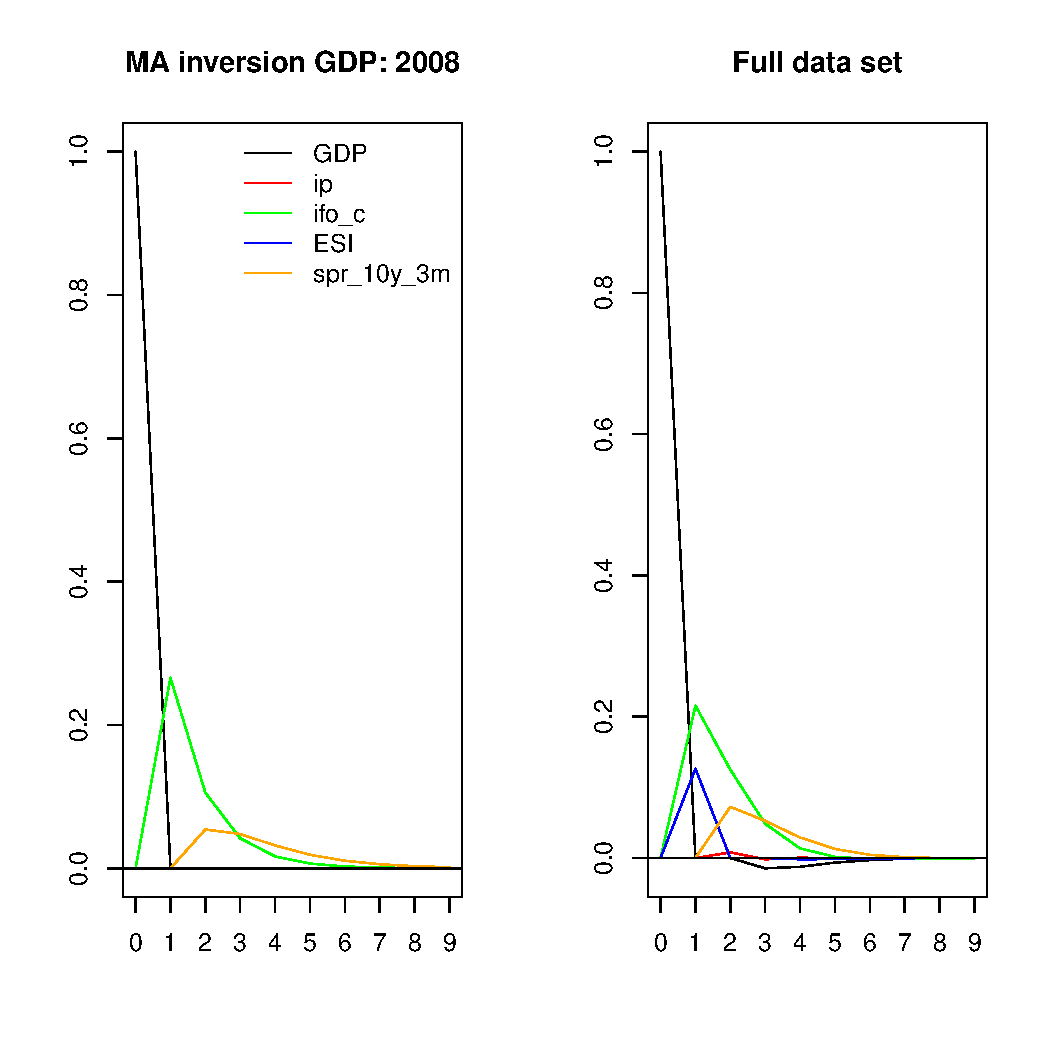
\includegraphics[height=3in, width=4.5in]{./Figures/up_dated_ma_inv_multi_ip.pdf}
        \caption{MA-inversion (impulse response) of VAR: data up to Q4-2007 (left) vs. entire data set without pandemic (right).
        \label{up_dated_ma_inv_multi_ip}}
    \end{center}
\end{figure}

\begin{figure}[h!]
    \begin{center}
        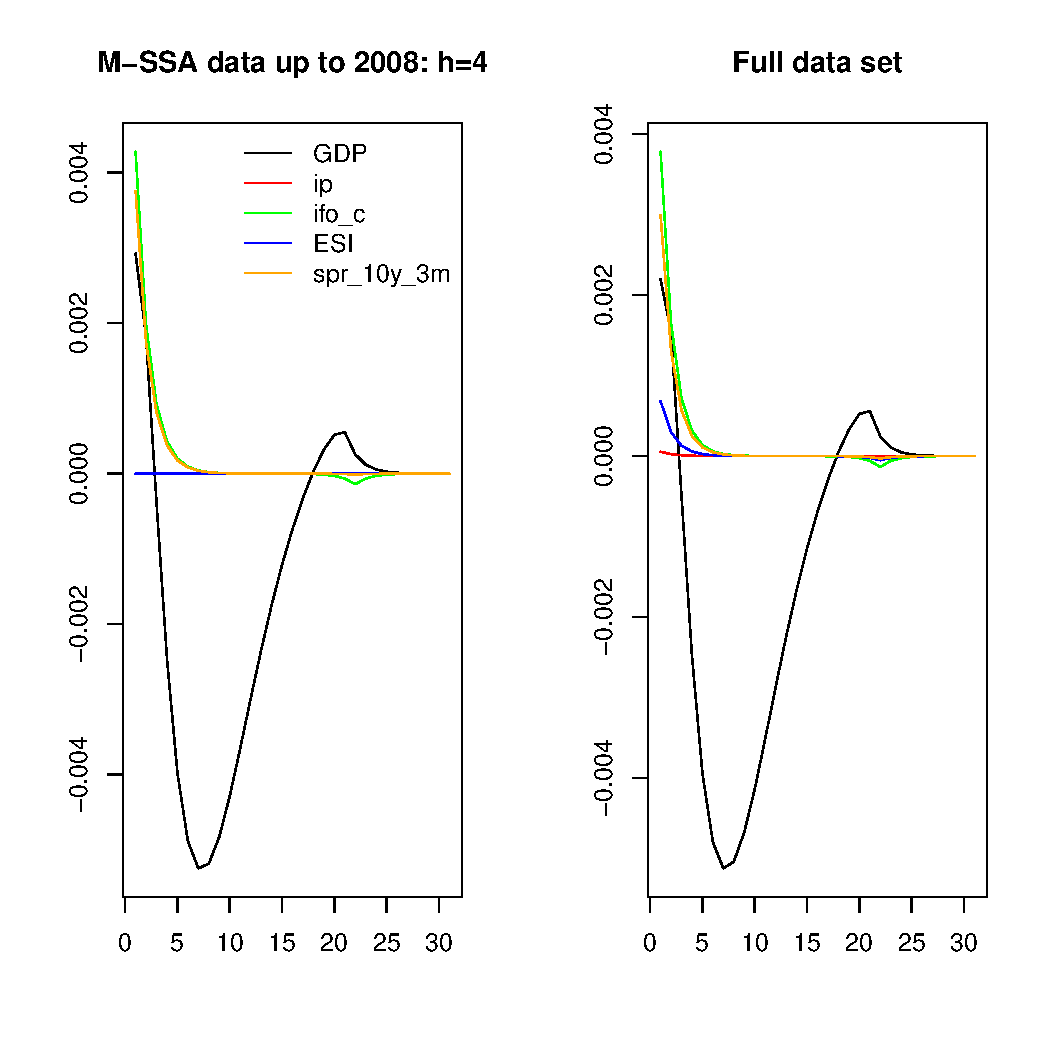
\includegraphics[height=3in, width=4.5in]{./Figures/bk_2008_all.pdf}
        \caption{M-SSA filter tracking HP-GDP at forecast horizon $h=4$: data up to Q4-2007 (left) vs. entire data set without pandemic (right).
        \label{bk_2008_all}}
    \end{center}
\end{figure}

\begin{figure}[h!]
    \begin{center}
        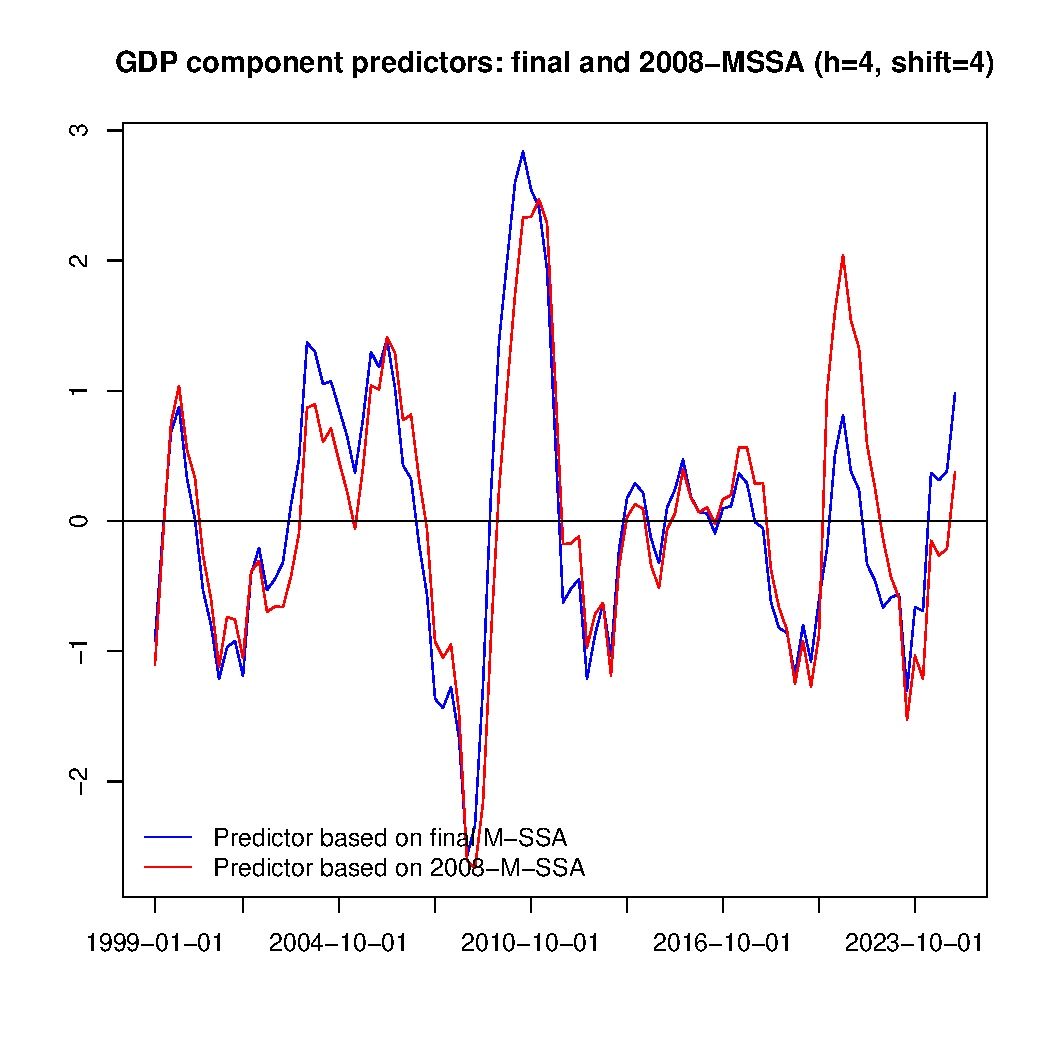
\includegraphics[height=3in, width=4.5in]{./Figures/revisions3.pdf}
        \caption{Revisions resulting from updates to the VAR model in M-SSA optimized for $h=shift=4$. To isolate the effect of the regression revision, all series are standardized. The up-dated M-SSA (blue) is left-shifted at the zero-crossings and appears slightly faster. For consistency, the entire pandemic episode has been removed.
        \label{revisions3}}
    \end{center}
\end{figure}

The second source of revisions in the M-SSA component predictor arises from updates to the VAR(1) model within the M-SSA filter\footnote{Similar findings apply to more sophisticated alternatives such as the VAR(3) discussed in Section \ref{sec:data}.}. We compare the original estimates, based on data up to Q4-2007, with the final estimates obtained using $h=4$ and $shift=4$ (similar findings apply to other values of forecast horizon and forward-shift).  For consistency, we excluded the entire pandemic episode from the data. Figure \ref{up_dated_ma_inv_multi_ip} compares the MA-inversions (impulse responses) of the GDP equation derived from the `old' and the updated VAR models: unlike the former, the latter incorporates ESI as an additional explanatory variable for GDP. Figure \ref{bk_2008_all} illustrates the resulting effect on the M-SSA filter targeting HP-GDP at forecast horizon $h=4$. The updated filter (right panel) assigns more weight to the additional `leading' indicators relative to GDP. Finally, Figure \ref{revisions3} compares the M-SSA GDP predictors. To isolate the effect of the regression revision, the figure displays standardized series. The update to the VAR model results in a leftward shift of the predictor (represented by the blue line), which appears marginally more rapid compared to the original predictor (depicted by the red line). It is important to note that the smoothness (zero-crossing rate) remains unchanged, though. 
This suggests that the out-of-sample performance of the M-SSA component predictor may be better than reported in Section \ref{oosp}, which is based on the fixed and increasingly outdated version of M-SSA.


\section{Summary and Conclusion}\label{sec:conclusions}


Classic direct forecasts of GDP can outperform simple benchmarks, such as the mean, up to two quarters ahead. However, this limited forecast horizon is often insufficient for certain applications. A key challenge with direct forecasts is that the relevant indicators tend to be noisy, which can mask the true signal and lead to overfitting, see \cite{Hastie2009}. In particular, the predictor struggles to timely track dips (slowdowns, recessions) or peaks (recoveries, expansions). To address this issue, we apply a HP(160)-filter to smooth the data, with the smoothing parameter $\lambda=160$ reflecting a more adaptive design than the classic quarterly HP, in line with an intended forecast horizon of up to one year ahead. The resulting predictor tends to outperform the classic direct forecasts in terms of statistical significance, mainly due to a slight left-shift noticeable at sharp recessions such as the Great Financial Crisis or Covid19-Pandemic. However, despite the filtering, the predictor remains somewhat noisy, potentially producing excessive noisy sign changes at (or in the vicinity of) the transitions between recessions and expansions. This issue is partly due to noise leakage inherent in the one-sided HP filter. \\

To address these problems, we propose a multivariate extension of the SSA framework based on \cite{Wildi2024}. Unlike the univariate HP filter, the M-SSA can leverage cross-sectional information from indicators leading GDP in real time while controlling for the rate of zero-crossings of the predictor. Consequently, the multivariate filter outputs become increasingly left-shifted as the forecast horizon lengthens, allowing dips and peaks of the target series to be tracked more systematically, while reducing the occurrence of noisy zero-crossings. However, since M-SSA does not explicitly target GDP, an additional step is necessary to derive the final GDP predictor.\\% We propose two approaches: a simple equally-weighted aggregate, assuming all M-SSA components are equally important for predicting GDP, and an optimally weighted predictor based on a regression of the M-SSA components on future GDP.\\

For illustration, we consider a simple approach based on regressing the single M-SSA GDP output on future GDP, thereby ignoring the other filter outputs. This predictor is intuitively appealing because the future HP-GDP, i.e., the target of M-SSA—is the low-frequency component of the future GDP target. Consequently, a strong link between M-SSA and future HP-GDP also indicates a connection with GDP, even if the statistical significance is obscured by the noise inherent in GDP. Out-of-sample performance suggests that this predictor is statistically significant at horizons exceeding one year. Moreover, designs optimized for larger forecast horizons outperform the mean benchmark at all considered forecast horizons, and the predictor exceeds the performance of direct forecasts---based on unfiltered or HP filtered indicators---at horizons longer than two quarters. An analysis of hit and false alarm rates within the ROC curve confirms that filtering improves predictive performance for forecast horizons exceeding two quarters. Multivariate approaches can further capitalize on leading indicators within the cross-sectional data. Additionally, the AUC is optimized through more precise control of the zero-crossing rate within the M-SSA framework. Finally, an examination of revision errors associated with quarterly updates of the proposed M-SSA-based GDP component predictor indicates that the regression parameters, VAR model, and resulting M-SSA filters stabilize after an initial burn-in period. This stabilization enhances the model’s explainability and interpretability.\\

In conclusion, the new predictor design integrates the traditional direct forecast approach with a novel multivariate filter to target quarterly GDP growth up to one year ahead. This multivariate approach leverages a set of economic indicators leading GDP in real time while controlling the smoothness of the predictor through the zero-crossing rate. 


%%%%%%%%%%%%%%%%%%%
%\newpage
\bibliographystyle{apalike}
\bibliography{references}
%%%%%%%%%%%%%%%%%%%%%%%%%%%
\newpage
\section{Appendix}\label{sec:Appendix}

\subsection{Additional Performances Results: Without Pandemic}


% latex table generated in R 4.2.2 by xtable 1.8-4 package
% Wed May  7 12:49:51 2025
% latex table generated in R 4.2.2 by xtable 1.8-4 package
% Wed May  7 12:49:51 2025
\begin{table}[ht]
\centering
\begin{tabular}{rrrrrrrr}
  \hline
 & h=0 & h=1 & h=2 & h=3 & h=4 & h=5 & h=6 \\ 
  \hline
Shift=0 & 1.131 & 1.092 & 1.028 & 0.973 & 0.977 & 1.040 & 1.119 \\ 
  Shift=1 & 1.295 & 1.274 & 1.206 & 1.106 & 1.039 & 1.044 & 1.097 \\ 
  Shift=2 & 1.180 & 1.194 & 1.178 & 1.109 & 1.029 & 0.990 & 0.997 \\ 
  Shift=3 & 1.029 & 1.061 & 1.082 & 1.051 & 0.984 & 0.936 & 0.923 \\ 
  Shift=4 & 1.012 & 1.057 & 1.100 & 1.096 & 1.036 & 0.967 & 0.924 \\ 
  Shift=5 & 0.988 & 1.033 & 1.076 & 1.084 & 1.048 & 0.987 & 0.929 \\  
   \hline
\end{tabular}
\caption{Regression of shifted GDP on M-SSA($h$) GDP component.\\rRMSEs benchmarked against the direct forecast.\\Out-of-sample evaluation starting in Q1-2008, without pandemic.} 
\label{rRMSE_mSSA_comp_direct_without_covid7}
\end{table}% latex table generated in R 4.2.2 by xtable 1.8-4 package
% Wed May  7 12:49:51 2025
\begin{table}[ht]
\centering
\begin{tabular}{rrrrrrr}
  \hline
 & Shift=0 & Shift=1 & Shift=2 & Shift=3 & Shift=4 & Shift=5 \\ 
  \hline
rRMSE & 0.862 & 0.838 & 0.912 & 1.008 & 1.001 & 1.028 \\  
   \hline
\end{tabular}
\caption{Direct forecasts.\\
rRMSEs benchmarked against the expanding mean.\\Out-of-sample evaluation starting in Q1-2008, without pandemic.} 
\label{rRMSE_mSSA_direct_mean_without_covid8}
\end{table}

\newpage
\subsection{Performances: Including Singular Pandemic Data}



% latex table generated in R 4.2.2 by xtable 1.8-4 package
% Wed May  7 12:49:51 2025
\begin{table}[ht]
\centering
\begin{tabular}{rrrrrrrr}
  \hline
 & h=0 & h=1 & h=2 & h=3 & h=4 & h=5 & h=6 \\ 
  \hline
Shift=0 & 0.080 & 0.042 & 0.011 & 0.001 & 0.000 & 0.002 & 0.011 \\ 
  Shift=1 & 0.403 & 0.297 & 0.188 & 0.095 & 0.042 & 0.039 & 0.103 \\ 
  Shift=2 & 0.718 & 0.594 & 0.359 & 0.114 & 0.019 & 0.009 & 0.022 \\ 
  Shift=3 & 0.955 & 0.950 & 0.871 & 0.569 & 0.158 & 0.031 & 0.013 \\ 
  Shift=4 & 0.593 & 0.879 & 0.957 & 0.893 & 0.541 & 0.183 & 0.080 \\ 
  Shift=5 & 0.531 & 0.875 & 0.971 & 0.929 & 0.605 & 0.239 & 0.041 \\ 
   \hline
\end{tabular}
\caption{p-values for $H_0: {\alpha_1} = 0$, HAC-adjusted Wald test, Equation \ref{eq_gdp_pred}.\\ including the pandemic.} 
\label{p_val1}
\end{table}% latex table generated in R 4.2.2 by xtable 1.8-4 package
% Wed May  7 12:49:51 2025
\begin{table}[ht]
\centering
\begin{tabular}{rrrrrrrr}
  \hline
 & h=0 & h=1 & h=2 & h=3 & h=4 & h=5 & h=6 \\ 
  \hline
Shift=0 & 0.999 & 0.980 & 0.951 & 0.925 & 0.915 & 0.926 & 0.955 \\ 
  Shift=1 & 1.057 & 1.051 & 1.028 & 0.996 & 0.977 & 0.978 & 0.985 \\ 
  Shift=2 & 1.031 & 1.035 & 1.026 & 0.996 & 0.964 & 0.952 & 0.964 \\ 
  Shift=3 & 1.022 & 1.035 & 1.042 & 1.026 & 0.992 & 0.965 & 0.953 \\ 
  Shift=4 & 1.002 & 1.023 & 1.044 & 1.046 & 1.024 & 0.999 & 0.984 \\ 
  Shift=5 & 1.010 & 1.032 & 1.054 & 1.060 & 1.043 & 1.013 & 0.983 \\  
   \hline
\end{tabular}
\caption{rRMSEs: out-of-sample forecast errors Equation \ref{oosfe} vs expanding mean of GDP\\Out-of-sample evaluation starting in Q1-2008, including the pandemic.\\Values $< 1$ indicate superior predictions from Equation \ref{oos_pred}.} 
\label{rRMSE_mSSA_comp_mean2}
\end{table}% latex table generated in R 4.2.2 by xtable 1.8-4 package
% Wed May  7 12:49:51 2025
\begin{table}[ht]
\centering
\begin{tabular}{rrrrrrrr}
  \hline
 & h=0 & h=1 & h=2 & h=3 & h=4 & h=5 & h=6 \\ 
  \hline
Shift=0 & 1.230 & 1.207 & 1.172 & 1.139 & 1.127 & 1.140 & 1.177 \\ 
  Shift=1 & 0.984 & 0.977 & 0.956 & 0.927 & 0.909 & 0.910 & 0.916 \\ 
  Shift=2 & 1.039 & 1.044 & 1.035 & 1.004 & 0.972 & 0.960 & 0.972 \\ 
  Shift=3 & 1.046 & 1.059 & 1.067 & 1.050 & 1.015 & 0.987 & 0.975 \\ 
  Shift=4 & 0.982 & 1.002 & 1.023 & 1.024 & 1.003 & 0.978 & 0.964 \\ 
  Shift=5 & 0.979 & 1.001 & 1.022 & 1.028 & 1.012 & 0.983 & 0.953 \\   
   \hline
\end{tabular}
\caption{Regression of shifted GDP on M-SSA($h$) GDP component.\\rRMSEs benchmarked against the direct forecast.\\Out-of-sample evaluation starting in Q1-2008, including the pandemic.} 
\label{rRMSE_mSSA_comp_direct3}
\end{table}% latex table generated in R 4.2.2 by xtable 1.8-4 package
% Wed May  7 12:49:51 2025
\begin{table}[ht]
\centering
\begin{tabular}{rrrrrrr}
  \hline
 & Shift=0 & Shift=1 & Shift=2 & Shift=3 & Shift=4 & Shift=5 \\ 
  \hline
rRMSE & 0.812 & 1.075 & 0.992 & 0.977 & 1.021 & 1.031 \\ 
   \hline
\end{tabular}
\caption{Direct forecasts.\\
rRMSEs benchmarked against the expanding mean.\\Out-of-sample evaluation starting in Q1-2008, including the pandemic.} 
\label{rRMSE_mSSA_direct_mean4}
\end{table}












\end{document}
